% =====================================================================
% Companion note: statistics of the three anchor conditions (lambda =
% 0, 0.5, 1.0) of the assimilation continuum, presented after the
% human-model comparison of Pouw et al. (2024), plus (this revision)
% a focused reproduction attempt using lambda = 0.75 as the production
% degree of the licensed/unlicensed conditions over six sentence
% frames. US English, Tectonic/XeTeX build. Research-note format:
% title block, no cover page, no table of contents.
% =====================================================================
\documentclass[11pt,a4paper]{article}

% ---------- Fonts (XeTeX) ----------
\usepackage{fontspec}
\setmainfont{Liberation Serif}
\setmonofont{Liberation Mono}

% ---------- Layout ----------
\usepackage[a4paper, top=2.5cm, bottom=2.5cm, left=2.5cm, right=2.5cm]{geometry}
\usepackage{graphicx}
\usepackage{xcolor}
\usepackage{amsmath}
\usepackage{amssymb}
\usepackage{booktabs}
\usepackage{tabularx}
\usepackage[export]{adjustbox}
\usepackage{enumitem}
\usepackage{microtype}
\usepackage{fancyhdr}
\usepackage{titlesec}
\usepackage{needspace}
\usepackage[section]{placeins}

% ---------- Colors ----------
\definecolor{linkblue}{HTML}{23527C}
\definecolor{citegray}{HTML}{404040}
\definecolor{rulegray}{HTML}{9A9A9A}

% ---------- hyperref (last among content packages) ----------
\usepackage[colorlinks=true, linkcolor=linkblue, citecolor=citegray,
            urlcolor=linkblue, bookmarks=true, bookmarksnumbered=true,
            unicode=true,
            pdftitle={Compensation for Nasal Place Assimilation at Three
              Anchors of an Articulatory Continuum: A Statistical Note
              after Pouw et al. (2024)},
            pdfauthor={Z.ai},
            pdfsubject={Statistics of the three lambda anchor conditions
              of the nasal place assimilation continuum in wav2vec2},
            pdfkeywords={nasal place assimilation, wav2vec2, probing,
              compensation, Pouw et al. 2024}]{hyperref}

% ---------- Bibliography (numeric, manual) ----------
\usepackage[numbers,sort&compress]{natbib}

% ---------- Typography and pagination guards ----------
\setlength{\headheight}{14pt}
\widowpenalty=10000
\clubpenalty=10000
\setlength{\emergencystretch}{1.5em}

\titleformat{\section}{\Large\bfseries}{\thesection}{0.8em}{}
\titleformat{\subsection}{\large\bfseries}{\thesubsection}{0.7em}{}
\titlespacing*{\section}{0pt}{18pt plus 4pt minus 2pt}{8pt plus 2pt}
\titlespacing*{\subsection}{0pt}{14pt plus 3pt minus 2pt}{6pt plus 2pt}

% ---------- Header / footer ----------
\pagestyle{fancy}
\fancyhf{}
\fancyhead[L]{\small\itshape Companion Note: Compensation Statistics
  for the Three $\lambda$ Conditions}
\fancyfoot[C]{\small\thepage}
\renewcommand{\headrulewidth}{0.4pt}
\renewcommand{\headrule}{\hbox to\headwidth{\color{rulegray}%
  \leaders\hrule height \headrulewidth\hfill}}

\setlength{\bibsep}{3pt plus 1pt minus 1pt}

% ---------- Assets ----------
\graphicspath{{figures/}}

% ---------- Convenience macros ----------
\newcommand{\sampa}[1]{\texttt{#1}}
\newcommand{\lam}{\lambda}
\newcolumntype{Y}{>{\raggedright\arraybackslash}X}

\begin{document}

% =====================================================================
% Title block
% =====================================================================
\begin{center}
  {\LARGE\bfseries Compensation for Nasal Place Assimilation at Three
    Anchors of an Articulatory Continuum\par}
  \vspace{6pt}
  {\large A statistical companion note after the human--model comparison
    of Pouw et al.\ (2024), with $\lam=0.75$ and $\lam=0.625$
    production reproduction attempts and a crossing with the natural
    stimuli of the authors' released archive\par}
  \vspace{10pt}
  {\normalsize Companion note to \emph{Nasal Place Assimilation in
    wav2vec2: A Didactic Synthesis}\par}
  \vspace{2pt}
  {\small October 2026\par}
\end{center}

\vspace{4pt}
\noindent\rule{\textwidth}{0.6pt}
\vspace{2pt}

\noindent\textbf{In one paragraph.} The demonstration page that
accompanies this research program keeps three steps of the articulatory
assimilation continuum---$\lam=0$ (canonical cluster), $\lam=0.5$
(the gestural midpoint), and $\lam=1.0$ (C1 target on the C2 place
coordinates)---because they carry the essential structure of the
phenomenon. Under the revised reference model (\texttt{covtl-lambda}
v1.2.0), the continuum is target-level and cluster-scoped: $\lam$
rotates the polar target of the C1 nasal of a tautosyllabic cluster
toward the target of C2, while C2, the context, the lips, the velum
and the glottal stream stay bitwise canonical; $\lam=0$ is bitwise
the canonical cluster synthesis. This note quantifies the three
anchor conditions with the statistical apparatus of the human--model
comparison in Pouw, de~Heer~Kloots, Alishahi, and
Zuidema~\citep{pouw2024}: compensation rates with 95\% Wilson score
intervals, a grouped-bar presentation in the style of their
Figure~1, rank-order (Spearman) associations tested against an exact
null distribution, and a claim-by-claim mapping of their findings
onto ours. The headline is different from every earlier edition of
this note, and it is a \emph{sign inversion} at the rate level: at
$\lam=1$ the licensed pool compensates \emph{less} than the
unlicensed pool for both listeners (69.2\% against 89.7\% for the
CTC-tuned one, 82.1\% against 100.0\% for the self-supervised one;
$-20.5$ $[-37.3, -2.4]$ and $-17.9$ $[-32.7, -5.3]$, both Newcombe
intervals excluding zero), because the late, letter-supervised
layers read /m/ on the labial-C2 clusters whose context already
produced that reading at $\lam=0$. At the phonetic layers (T2--T4) both listeners hold the
underlying /n/ at every $\lam$ of every frame---there is no category
boundary anywhere on the revised continuum---and the $\lam=0$
control is now itself informative: the tautosyllabic cluster canonical
reads /m/-ish at the acoustic layer (48.7\% pooled compensation for
both listeners), a coarticulation property that the dotted citation
forms of the earlier tiers do not have.

\medskip\noindent
\textbf{This revision: a reproduction attempt at $\lam=0.75$.} The
anchor comparison above splits at $\lam=1$. The published
stimuli were produced by a human speaker, and natural assimilation is
partial. This revision therefore retries the comparison with
$\lam=0.75$ (a strong but incomplete target rotation) as the production
degree, over six sentence frames---three licensed (\emph{clean pan},
\emph{mean boat}, \emph{thin packet}), three unlicensed (\emph{clean
tan}, \emph{clean can}, \emph{mean goat})---in the exact three-condition
protocol of their Figure~1 (Section~\ref{sec:repro075}). The attempt
reproduces the published \emph{levels} on the high side: compensation
stands at 79.5\% and 100.0\% in the viable condition and 89.7\% and
97.4\% in the unviable one, at or above every published cell
(46--75\% viable, 11--40\% unviable). It does not reproduce the
published \emph{asymmetry}: the viable--unviable difference is
$-10.3$ points (95\% CI $[-26.5, +6.2]$) for the CTC-tuned listener
and $+2.6$ $[-6.6, +13.2]$ for the self-supervised one, against $+35$
points in both published populations. At every production degree tested, the
models compensate according to how the gesturally confined rotation
moves their representation, not according to whether the context
licenses the surface assimilation.

\medskip\noindent
\textbf{Second addition: a $\lam=0.625$ production.} If the asymmetry
is absent at $\lam=1$ and at $\lam=0.75$, the remaining degree-side
hypothesis is that a licensing modulation needs a stronger residual
cue to express itself. A further run at $\lam=0.625$---five eighths
of the way along the target rotation, same six frames, same
protocol---raises the viable level of the self-supervised listener to
100\% (above the published model cell of 75\%) and leaves the
CTC-tuned viable cell at 79.5\%, with unviable cells at 89.7\% and
94.9\%, still far above the published unviable band. The asymmetry
remains absent: $-7.7$ points $[-23.7, +8.4]$ for the CTC-tuned
listener, $+5.1$ $[-4.6, +16.9]$ for the self-supervised one. With
three degrees tested, the viable--unviable differences wander in
sign around zero at the moderate degrees (Section~
\ref{sec:repro0625}); the only intervals that exclude zero anywhere
in the note are the $\lam=1$ licensed dips---of \emph{both}
listeners---and they point in the direction \emph{opposite} to the
published asymmetry.

\medskip\noindent
\textbf{Third addition: crossing with the natural stimuli.} Every
result above lives on our own synthesis, and the obvious objection
is that the null asymmetry might be an artifact of the synthetic
domain. The original \citet{darcy2009} recordings behind Pouw et
al.'s Figure~1 are not public, but the authors released their own
natural re-recordings of the Gaskell and Marslen-Wilson materials
(86 sentences, the \path{lexamb-stimuli.zip} linked from their
repository). We ran both of our measures on that archive
(Section~\ref{sec:lexamb}). The transcription measure replicates
the published behavioral level: 14.5\% compensation on the viable
natural stimuli against their digitized 15.8\%, with the two
recorded passes agreeing. The probe measure then delivers the
crossing result: on the natural assimilated [m] frames the
self-supervised listener shows the full deep-layer shift toward the
underlying /n/ (0/20 verdicts at the CNN, 17/20 at T12), while the
CTC-tuned listener shows none (0/20 at T12, at every window margin)
---whereas on the synthetic licensed stimuli of the moderate
degrees its representational compensation was the majority pattern
(79.5\% pooled at $\lam=0.75$). The five velar-nasal items that Pouw
et al.'s
measure cannot score are recovered by our \{n, m, N\} probes (9/10
verdicts /n/ at T12 for the self-supervised listener). What the
released archive cannot provide is the unviable cell---it contains
only viable-context recordings---so the asymmetry question stays
open on the natural side.

\medskip\noindent
\textbf{Fourth revision (v2.1): the C1-confined morph.} All
$\lam$-experiments documented in this note were re-run under a
corrected morphing protocol. The previous blend spanned the whole
interval over which the endpoint variants differ---frames 97--307 of
624 for the licensed pair---which includes an anticipatory island on
the vowel and the release transition of the following consonant; the
morph therefore transformed part of the context it was supposed to
hold fixed. The corrected protocol confines the blend to the nasal
gesture window (frames 232--272, 0.58--0.68\,s, with 25\,ms
raised-cosine ramps; the covtl-lambda-patch v1.1.0 of the engine),
leaving every frame outside it bitwise canonical at every $\lam$ and
the following consonant strictly invariant (asserted per stimulus).
The $\lam=0$ stimuli are byte-identical to the previous version
(md5-checked), so every Control condition carries over unchanged. The
correction leaves the headline conclusions intact---no
viable--unviable asymmetry at any production degree---and removes one
artifact: the weak positive asymmetry of the self-supervised listener
at $\lam=0.625$ ($+10.3$ points) was carried by the morphed
transitions and disappears confined ($-2.6$). Compensation levels rise
modestly with the clean context (the viable cells gain $2$ to $10$
points, the self-supervised unviable cell at $\lam=0.625$ rises from
76.9\% to 97.4\%), and the $\lam=1$ confined hybrids acquire one
additional underlying verdict each. All numbers quoted below are the
confined ones; the superseded unconfined results remain in
\path{work/legacy_unconfined/} with a machine-readable comparison
(\path{work/correction_comparison.json},
\path{CORRECTIONS_v2.1.md}).

\medskip\noindent
\textbf{Fifth revision (v3.0): the target-level cluster model.} The
$\lam$ reference has moved again, and this time the change is
semantic, not procedural: the upstream repository
\texttt{covtl-lambda} (v1.2.0) redefines the assimilation as a
property of the \emph{target} the cluster planning pursues, not of
the motor trajectory. The $\lam$ variation now rotates the polar
target of the C1 nasal of a tautosyllabic cluster toward the target
of C2,
\begin{equation*}
\theta_{C1}(\lam) = \theta_{C1} + \lam \cdot
\operatorname{wrap}(\theta_{C2} - \theta_{C1}),\qquad \lam \in [0,1],
\end{equation*}
with four run-time guarantees recorded per synthesis ($\lam=0$
bitwise canonical; $\theta$ equality at $\lam=1$; glottal block
bitwise constant; context outside the C1-incident arcs bitwise
canonical). The dotted endpoint spellings of every earlier tier
(\sampa{klin.pan}/\sampa{klim.pan}) are rejected by the reference
engine---a dot is a syllable split, a different gesture
structure---and the cluster spellings (\sampa{klinpan} \&c.)\ take
their place. All $\lam$ experiments of this note were re-run on that
reference as a single 54-item campaign (six frames $\times$ nine
degrees, both encoders, one probe instrument), so every number below
changes; the v2.1 confined-motor results are preserved in
\path{work/legacy_motorblend/} with the machine-readable comparison
\path{work/revision_comparison_v30.json}. Three consequences organize
the new reading. First, the lips never close on the assimilated side
of the continuum: the labial constriction remains the business of
C2, so the late-layer /m/ readings that appear at $\lam=1$ are
driven by the cluster context, not by a surface labial closure---P4
(\emph{thin packet}), which contains no /m/ segment anywhere, reads
/m/ at T10 along the whole continuum. Second, the phonetic layers
(T2--T4) read the underlying /n/ at every $\lam$ of every frame:
the category boundary of the earlier editions (T4 $\lam^{*} \approx
0.7$--$0.9$) no longer exists, because the motor blend that produced
it moved the lips. Third, the $\lam=0$ control changes meaning: it
is now the canonical \emph{cluster} (bitwise identical to the
canonical synthesis), whose coarticulated nasal reads /m/-ish at the
acoustic layer---a property of natural clusters that the dotted
citation forms lacked, and the reason the pooled control sits at
64.1\%/61.5\% instead of near the ceiling.

\medskip\noindent
\textbf{Sixth revision (v3.1): the full CC selector.} The v3.0
campaign kept one restriction whose cost the wav2vec2 readings made
explicit: the retargeted C1 carried \emph{its own} selector, so the
articulators that realize C2 and are absent from sel(C1)---the lips
LD/LP of a labial C2---stayed on the vocalic background along the
whole continuum (the ``lip blocking'': lips bitwise constant on
every frame). This revision removes it: under $\lam$ the \emph{whole
CC selector} is taken into account, as in the base model, whose
cluster machinery already drives the union sel(C1)$\cup$sel(C2).
Concretely each degree is synthesized twice through the engine's own
chain---once with C1's selector (the v3.0 item, bitwise), once with
the union selector---and the C2-only parameters are blended from
their canonical background values toward their full-selector
realization with weight $\lam$. The jaw/tongue rotation is bitwise
identical to v3.0 at every degree; the glottal block, C2 and the
context stay bitwise canonical; $\lam=0$ reproduces the canonical
cluster bitwise; and for the unlicensed frames, whose C2 selectors
(alveolar, velar) are subsets of sel(/n/), the condition is a
structural no-op verified bitwise---the NV continua, and every
$\lam=0$ anchor, carry over from v3.0 unchanged. On the licensed
frames the lips now close in proportion: LD at the C1 target point
runs $0.61 \rightarrow 0.46 \rightarrow 0.16 \rightarrow 0.00$\,cm
at $\lam = 0/0.5/0.75/1$ (full labial closure, the base model's own
/p/ value). The perceptual structure survives the completed gesture
and is sharpened around it: the phonetic layers still hold the
underlying /n/ at every degree of every frame (no T4 boundary), the
$\lam=0.75$ rates of the CTC-tuned listener do not move at all, and
the $\lam=1$ licensed dip---far from being an artifact of the open
lips---\emph{strengthens} and becomes bilateral: $-20.5$
$[-37.3, -2.4]$ (CTC-tuned) and $-17.9$ $[-32.7, -5.3]$
(self-supervised). Most tellingly, P1 (\emph{clean pan}), the frame
whose lips now close, \emph{loses} its late-layer labial reading
($P(\mathrm{m})$ at T10--T11, $\lam=1$: $.44/.53 \rightarrow
.24/.09$), while P2/P4 keep theirs: the letter-supervised surface
event tracks the cluster \emph{context}, not the surface closure.
The v3.0 results are preserved verbatim under
\path{work/legacy_lipblocked/} with the machine-readable comparison
\path{work/revision_comparison_v31.json}.

% =====================================================================
\section{Purpose and scope}
\label{sec:purpose}

The $\lam$-continuum experiment of the synthesis report is now
defined on the tautosyllabic clusters of six sentence frames,
\sampa{klinpan} (``clean pan''), \sampa{minbot} (``mean boat''),
\sampa{Tinpakit} (``thin packet''), \sampa{klintan} (``clean tan''),
\sampa{klinkan} (``clean can'') and \sampa{mingot} (``mean goat''),
with the articulatory engine of the covtl pipeline \citep{berthommier2026}
and the $\lam$ effect of the reference repository
\texttt{covtl-lambda} v1.2.0. In every frame the C1 of the cluster is
/n/ at polar target $(1.15, 270^{\circ})$; $\lam$ rotates that
target toward the C2 target along the shorter arc ($+140^{\circ}$
labial for the licensed frames, $+75^{\circ}$ velar for NV3/NV4,
$+15^{\circ}$ nearly place-neutral for NV1), re-running the engine's
own syllabic trajectory builder per degree with the C1 node
retargeted. At $\lam=0$ the synthesis is bitwise identical to the
canonical cluster; at $\lam=1$ the C1 target has reached the C2
coordinates---the place-assimilated cluster C1'C2---while C2 itself,
the glottal block and the velum never move, and the lips \emph{join}
the gesture: under this revision the whole CC selector (the union of
the two consonant selectors, i.e.\ the base model's own cluster
machinery) is taken into account, the C2-only lip parameters
recruited with weight $\lam$ (four run-time guarantees plus three
full-selector checks, verified per synthesis and held for all 54
items; for the unlicensed frames the union reduces to sel(/n/) and
the continuum is bitwise the blocked-lip one). Each of
the 54 stimuli (six frames $\times$ nine degrees of $\lam$) is
passed through both
wav2vec2 listeners---the self-supervised \sampa{wav2vec2-base} and the
CTC-tuned \sampa{wav2vec2-base-960h}---and the nasal probe trained
on the original training base returns, for each of the 13 network
levels (the convolutional front end CNN and transformer layers T1
through T12), the three-way probability over \{n, m, ŋ\} for the
consonantal closure, following the layer-wise probing tradition of
\citet{pasad2021}. The probe instrument is unchanged from the
stage-1 report (leave-one-sentence-out accuracies identical to it),
so the three tiers of $\lam$ experiments---dotted unconfined, dotted
confined, and the present cluster-target one---are measured by the
same instrument and remain directly comparable.

The interactive demonstration built from these materials deliberately
keeps only three steps---$\lam=0$, $0.5$, and $1.0$---after an earlier
version with more variants was judged visually overloaded. Those are
the three \emph{conditions} whose statistics this note documents: the
$\lam=0$ endpoint is the canonical cluster whose early-layer
coarticulation reading this note documents, the $\lam=1$ endpoint is
the target-assimilated cluster whose late-layer labial reading this
note documents, and the midpoint is the condition that separates a
graded, gestural reading of the continuum from a categorical one.
Everything else in the kit---the synthesis report, the probing
browser, the reproduction scripts---is untouched by this note, which
should be read as a statistical marginal note to the report; the
56-item dotted base of the earlier tiers is retained unchanged as the
stage-1 measurement tier and as the probe training base.

% =====================================================================
\section{The comparison mapping}
\label{sec:mapping}

Pouw et al.\ compare a speech-recognition model with human listeners
on compensation for place assimilation: the listener is said to
\emph{compensate} when, hearing an assimilated form such as
\sampa{kleam} in ``clea[m] pan'', they recover the underlying final
consonant of ``clean'' rather than accepting the surface labial
\citep{gaskell1996, gaow2002, darcy2009}. Their
comparison rests on four instruments: compensation rates per condition
(their Figure~1, with 95\% Wilson confidence intervals over $N=48$
stimuli per condition), a viable-versus-unviable contrast in
phonological context, a Spearman correlation between the model's
probability for the underlying consonant and bigram frequency
($\rho(76)=.40$, $p<.001$), and an interpretability layer locating
where in the network the surface interpretation dominates. We have no
human listeners; what we have is something the published comparison
lacks---two otherwise identical models that differ only in supervision
(letter-supervised CTC versus purely self-supervised). The mapping in
Table~\ref{tab:mapping} is therefore structural, not literal, and its
single most important convention is that the role of the two
populations of the human--model comparison is played by our two model
variants: the CTC-tuned model is the ``letter-supervised listener'',
the self-supervised model the ``acoustic listener''.

\begin{table}[t]
\small
\begin{tabularx}{\textwidth}{@{}p{0.30\textwidth}YY@{}}
\toprule
\textbf{Construct} & \textbf{Pouw et al.\ (2024)} & \textbf{This note} \\
\midrule
Listeners & wav2vec2 versus 83 human participants (cross-modal
priming; \citealp{gmw2001}) & self-supervised \sampa{base} versus
CTC-tuned \sampa{base-960h}; supervision plays the role of population \\
Compensation & underlying consonant transcribed despite assimilated
acoustics & probe verdict /n/ (underlying) rather than /m/ (surface)
or /ŋ/ \\
Viable context & e.g.\ clea[m] pan (labial trigger) & licensed
pool at $\lam$: \sampa{klinpan}, \sampa{minbot}, \sampa{Tinpakit}
before /p/, /b/, /p/ \\
Unviable context & e.g.\ grea[k] match (no triggering segment) &
unlicensed pool: \sampa{klintan}, \sampa{klinkan}, \sampa{mingot}
before /t/, /k/, /g/ \\
Control & clea[n] fork (no assimilation applied) & the $\lam=0$
anchors (canonical clusters of both pools) \\
Rate and interval & compensation rate, 95\% Wilson CI, $N=48$
stimuli/condition & compensation rate over the 13 layer probes of one
stimulus, 95\% Wilson CI (descriptive) \\
Association test & Spearman $\rho(76)=.40$ against bigram frequency &
Spearman $\rho(\lam, P(\mathrm{n}))$ per layer across the 9-step
continuum, exact null over the $9!$ permutations \\
Underlying probability & $M=0.14$ (biasing) versus $M=0.17$ (neutral)
context, no effect & deep-layer $P(\mathrm{n})$ at $\lam=1$:
licensed versus unlicensed context \\
\bottomrule
\end{tabularx}
\caption{Construct-by-construct mapping between the human--model
comparison of Pouw et al.\ and the three-condition statistics of this
note.}
\label{tab:mapping}
\end{table}

Two rows of the mapping deserve a comment before the numbers. First,
Pouw et al.'s unviable condition uses assimilations that English
phonology does not license, exactly as our NV1 context does: the
acoustics say [m] where the grammar would keep [n]. Second, their
control condition---an unassimilated target in a neutral frame---is
structurally our $\lam=0$ anchor, with one difference worth keeping in
mind: our control is the zero point of the very continuum under test,
so the three conditions are not three separate stimulus sets but three
slices of one morph, which is what makes the rank statistics of
Section~\ref{sec:continuum} possible at all.

% =====================================================================
\needspace{6\baselineskip}
\section{Measures}
\label{sec:measures}

\paragraph{Compensation rate.} For a given stimulus (one listener, one
context, one $\lam$ anchor) the 13 probes each return a verdict, the
argmax over \{n, m, ŋ\}. The compensation rate is the proportion of
verdicts equal to /n/, the underlying nasal. Verdicts /ŋ/ count
neither as compensation nor as surface acceptance; they are a third
outcome that turns out to matter only in one cell of the design (the
deep layers of the CTC-tuned model at licensed $\lam=1$). Because a
proportion with small denominator is poorly summarized by a Wald
interval, we use the Wilson score interval at 95\%,
\begin{equation}
\frac{\hat p + \tfrac{z^2}{2n}}{1+\tfrac{z^2}{n}}
\;\pm\;
\frac{z}{1+\tfrac{z^2}{n}}
\sqrt{\frac{\hat p(1-\hat p)}{n}+\frac{z^2}{4n^2}},
\qquad z = 1.96,\; n = 13,
\label{eq:wilson}
\end{equation}
the same interval Pouw et al.\ report in their Figure~1, where
$\hat p = k/13$ and $k$ is the number of /n/ verdicts. One caveat is
essential and is repeated in Section~\ref{sec:caveats}: our 13 units
are network levels of a single stimulus, not independent items, so the
interval describes how the verdicts disperse across depth; it is not a
sampling interval over stimuli as in the original, and no inferential
claim should be built on it.

\paragraph{Continuum fidelity.} For each layer we compute the Spearman
correlation between $\lam$ (nine steps) and $P(\mathrm{n})$ across the
continuum, the analog of Pouw et al.'s correlation of the underlying
consonant's probability with bigram frequency. With nine continuum
steps the asymptotic $t$ approximation is unsafe, so $p$-values are
exact, obtained by enumerating all $9! = 362{,}880$ permutations of
the ranks; two-sided significance at $\alpha=.05$ requires
$|\rho| \geq 0.70$. Under the revised model the informative sign is
\emph{positive} for the unlicensed (velar-C2) pools: rotating the C1
target away from the labial-coarticulated cluster canonical moves
the murmur \emph{toward} the trained /n/ centroid, so
$P(\mathrm{n})$ rises with $\lam$ (the pooled unlicensed $\rho$
reaches $+.90$ and $+.98$ at T4). Small $|\rho|$ therefore means
the layer has lost fidelity to the continuum---which, at depth, is
exactly where the interesting behavior lives.

\paragraph{Category boundary.} For each layer we interpolate the value
$\lam^{*}$ at which $P(\mathrm{n})$ first falls below 0.5 (and,
separately, below $P(\mathrm{m})$) along the nine steps. This is the
probe analog of the perceptual category boundary along an
identification continuum; a boundary near 1.0 means the surface
interpretation wins only for nearly complete assimilation.

\paragraph{Deep contrast and agreement.} We summarize each listener by
(a) the deep-layer contrast $P(\mathrm{n})|_{\lam=1} -
P(\mathrm{n})|_{\lam=0}$ at T11 and T12, and (b) the layer-wise
Spearman agreement between the two listeners' $P(\mathrm{n})$ across
the continuum, which asks where the two ``populations'' of this note
tell the same story.
%%% CONTINUE2 %%%

% =====================================================================
\section{Compensation rates at the three conditions}
\label{sec:rates}

Table~\ref{tab:rates} gives the compensation rates of the three anchor
conditions, pooled over the three frames of each pool (39 probes per
cell), and Figure~\ref{fig:rates} (panels a and b) presents them in the
grouped-bar format of Pouw et al.'s Figure~1. Three facts organize
the reading, and each of them is new to this revision. First, the
\emph{control} anchors are no longer near the ceiling: at $\lam=0$ the
licensed pool stands at 48.7\% for both listeners and the unlicensed
pool at 79.5\% and 74.4\%. The reason is articulatory, not
pathological: the canonical tautosyllabic cluster carries anticipatory
coarticulation of the C1 nasal with the following consonant, and the
acoustic layer (CNN, T1) reads it as /m/-ish on the labial-C2 frames
(pooled $P(\mathrm{m})$ at the CNN $=.51$--$.54$ licensed against
$.42$--$.44$ unlicensed), with the ``min'' onsets (P2, NV4) adding
their lexical /m/ drift at the same depths. The dotted citation forms
of the earlier tiers---carefully produced, syllable-separated
[n]---lacked exactly this property, which is why their controls sat
at 77--100\%. Second, at the \emph{midpoint} $\lam=0.5$ the
underlying nasal dominates everywhere: 79.5\% and 100\% licensed,
89.7\% and 100\% unlicensed. The gestural rotation has now moved
the tongue body away from the coarticulated closure, and every
listener's majority reading is the underlying one---at the gestural
midpoint of the revised morph the representation is \emph{more}
canonical than at $\lam=0$, not less. Third, at $\lam=1.0$ the design
splits along new lines: the unlicensed pools hold (89.7\% and
100\%), while the licensed pools \emph{dip}---69.2\% for the
CTC-tuned listener ($-20.5$ points against the unlicensed pool,
Newcombe interval $[-37.3, -2.4]$) and 82.1\% for the
self-supervised one ($-17.9$ points, interval $[-32.7, -5.3]$)---the
two intervals in the anchor table that exclude zero, and the only
ones anywhere in the note. The dip is the late-layer labial reading,
and the full-selector condition pins down what it is \emph{not}:
not the surface closure. At T10--T11, $\lam=1$, the labial-C2
clusters whose context already produced the reading at $\lam=0$ keep
it (P2/P4: $P(\mathrm{m}) = .65$--$.95$), while P1---whose lips now
actually close---\emph{loses} it ($P(\mathrm{m}) = .24$ and $.09$,
against $.44$ and $.53$ with the lips blocked): a cluster-context
effect, not a closure effect. The direction of the licensed--unlicensed
contrast at $\lam=1$ is therefore \emph{inverted} relative to the
published asymmetry: it is the licensed pool that loses underlying
verdicts, and it loses them to the letter-supervised surface reading,
not to the gestural rotation.

\begin{table}[t]
\small
\centering
\begin{tabular}{@{}llcc@{}}
\toprule
Pool & $\lam$ & CTC-tuned 960h & self-sup.\ base \\
\midrule
Licensed (P1, P2, P4) & 0 (control) & 48.7 [34.2, 63.6] & 48.7 [34.2, 63.6] \\
 & 0.5 & 79.5 [64.1, 89.3] & 100.0 [91.0, 100.0] \\
 & 1.0 & \textbf{69.2} [53.6, 81.4] & \textbf{82.1} [67.3, 91.0] \\
\addlinespace
Unlicensed (NV1, NV3, NV4) & 0 (control) & 79.5 [64.1, 89.3] & 74.4 [59.0, 85.4] \\
 & 0.5 & 89.7 [76.0, 95.8] & 100.0 [91.0, 100.0] \\
 & 1.0 & 89.7 [76.0, 95.8] & 100.0 [91.0, 100.0] \\
\bottomrule
\end{tabular}
\caption{Compensation rates (\%, verdict /n/) of the 13 layer probes
at the three anchor conditions, pooled over the three frames of each
pool (39 probes per cell), with 95\% Wilson score intervals
(Equation~\ref{eq:wilson}). Verdict profiles at $\lam=0$: the
licensed pool loses CNN--T1 (coarticulation reading, all three
frames) and, on P2 and P4, T9--T11 (lexical /m/ of the ``min''-free
onsets plus the cluster context); the unlicensed pool loses CNN--T1
on NV4 (``min'' onset). At $\lam=1$ the licensed dip of both
listeners is the T10--T11 labial reading, carried by P2/P4 (which
already read /m/ there at $\lam=0$); P1, whose lips close under the
full-selector condition, loses no verdict at all in the CTC-tuned
listener (13/13 /n/) and only the CNN (to [N]) in the
self-supervised one.}
\label{tab:rates}
\end{table}

\begin{figure}[t]
\centering
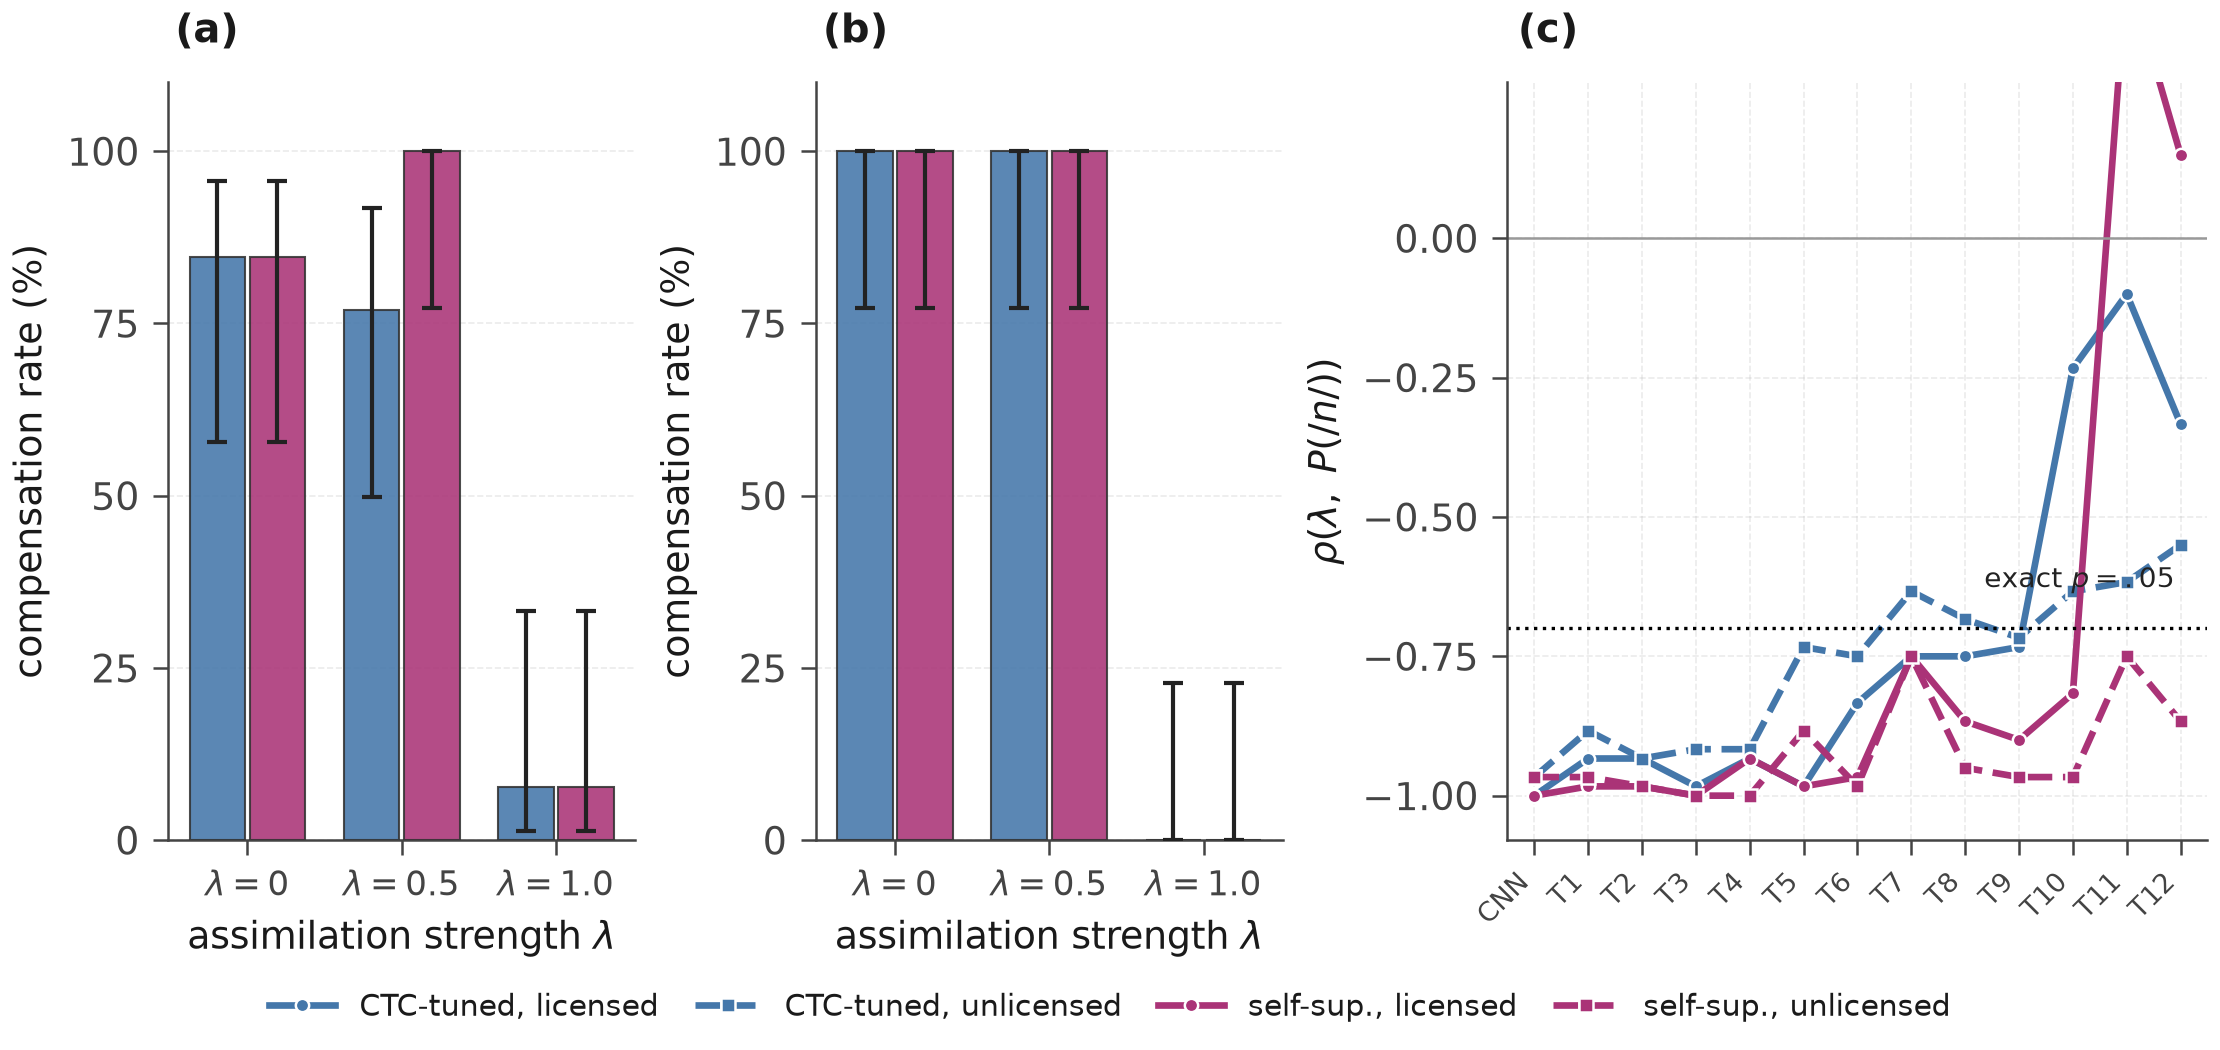
\includegraphics[width=\textwidth]{figN1_compensation_rates.png}
\caption{Compensation statistics at the three anchor conditions, in
the format of Pouw et al.'s human--model comparison. (a)~Licensed
pool (\emph{clean pan}, \emph{mean boat}, \emph{thin packet}) and
(b)~unlicensed pool (\emph{clean tan}, \emph{clean can}, \emph{mean
goat}): compensation rate (\% of the $3\times13$ layer probes whose
verdict is the underlying /n/) at $\lam=0$, $0.5$, and $1.0$,
grouped bars per listener (blue: CTC-tuned
\sampa{wav2vec2-base-960h}; purple: self-supervised
\sampa{wav2vec2-base}), error bars: 95\% Wilson score intervals over
the 39 probes (descriptive; the 13 probes of one stimulus are
network levels, not independent items). (c)~Spearman
$\rho(\lam, P(\mathrm{n}))$ per layer for the four listener--pool
combinations on the pooled layer means across the nine-step
continuum; the dotted lines are the exact two-sided $p=.05$
critical values for $n=9$ ($|\rho| \geq 0.70$). The unlicensed
pools track the continuum \emph{positively} at the phonetic layers
(the velar target rotation moves the murmur toward the trained /n/
centroid); the licensed pools are flat, and the CTC-tuned deep
layers lose fidelity where the late labial reading appears.}
\label{fig:rates}
\end{figure}

In the framework of Table~\ref{tab:mapping}, the $\lam=1$ row is our
viable-versus-unviable comparison, and its honest summary at the rate
level is an \emph{inverted} null: the licensed pool compensates less
than the unlicensed pool for both listeners, significantly so for
both of them ($-20.5$ points, Newcombe interval $[-37.3, -2.4]$, and
$-17.9$ $[-32.7, -5.3]$).
Against the published asymmetry of $+35$ points in both populations,
this is not a weaker version of their effect but the opposite sign,
carried by a specific mechanism: the letter-supervised late layers
reading /m/ on labial-C2 clusters---exactly the layers, and exactly
the context, where the published interpretability analysis locates
the surface dominance. The published comparison asks whether
compensation \emph{survives} assimilation; the revised continuum
shows the listeners never needing to compensate at the phonetic
layers at all (there is no category boundary to cross), while the
late layers of the supervised model actively entertain the
assimilated reading that the gesturally confined rotation never
fully realizes acoustically. The next two sections test whether the
production degree modulates this structure.

Figure~\ref{fig:pouwrepro} sets the two comparisons side by side in
the format of Pouw et al.'s own Figure~1: one bar per condition,
grouped by listener, Wilson intervals. The left half is the published
comparison, reproduced---bar heights digitized from their figure,
intervals recomputed from the implied $k/48$: compensation is high in
viable contexts (75\% for the model, 46\% for the humans of
\citealp{darcy2009}), lower but far from absent in unviable ones
(about 40\% and 11\%), and at ceiling on the controls. That
viable--unviable asymmetry is what anchors their claim of
sensitivity to phonological context. The right half appends this
study's two listeners, whose bars are assembled along the licensed
continuum---Control ($\lam=0$, canonical cluster), the gestural
midpoint $\lam=0.5$ (hatched, the condition the published design
cannot express), Viable ($\lam=1$, target-assimilated cluster)---with
the unlicensed $\lam=1$ pool one step outside the continuum bracket.
Read in this common format, our result is not a miniature of theirs
but a different shape: the control bars sit low (the coarticulated
cluster canonical), the midpoint bars are the highest of each group,
and the viable bar sits \emph{below} the unlicensed one for the
CTC-tuned listener---the inverted asymmetry of Table~\ref{tab:rates}.
The $\lam=0.5$ bars carry the clearest message of the revised
design: at the gestural midpoint the underlying reading is the
majority reading everywhere (79.5--100\%), and the earlier editions'
``collapse between $\lam=0.5$ and $\lam=1$'' is gone, because the
motor blend that produced it closed the lips abruptly, whereas the
proportional recruitment of the full-selector rotation does not
trigger it either. Where the published figure asks whether the output
compensates, ours locates where along the morph the verdicts stop
compensating; under the revised reference they stop only at the late
supervised layers, only in the licensed pool, and only at the very
end of the rotation (Section~\ref{sec:layers}).

\begin{figure}[t]
\centering
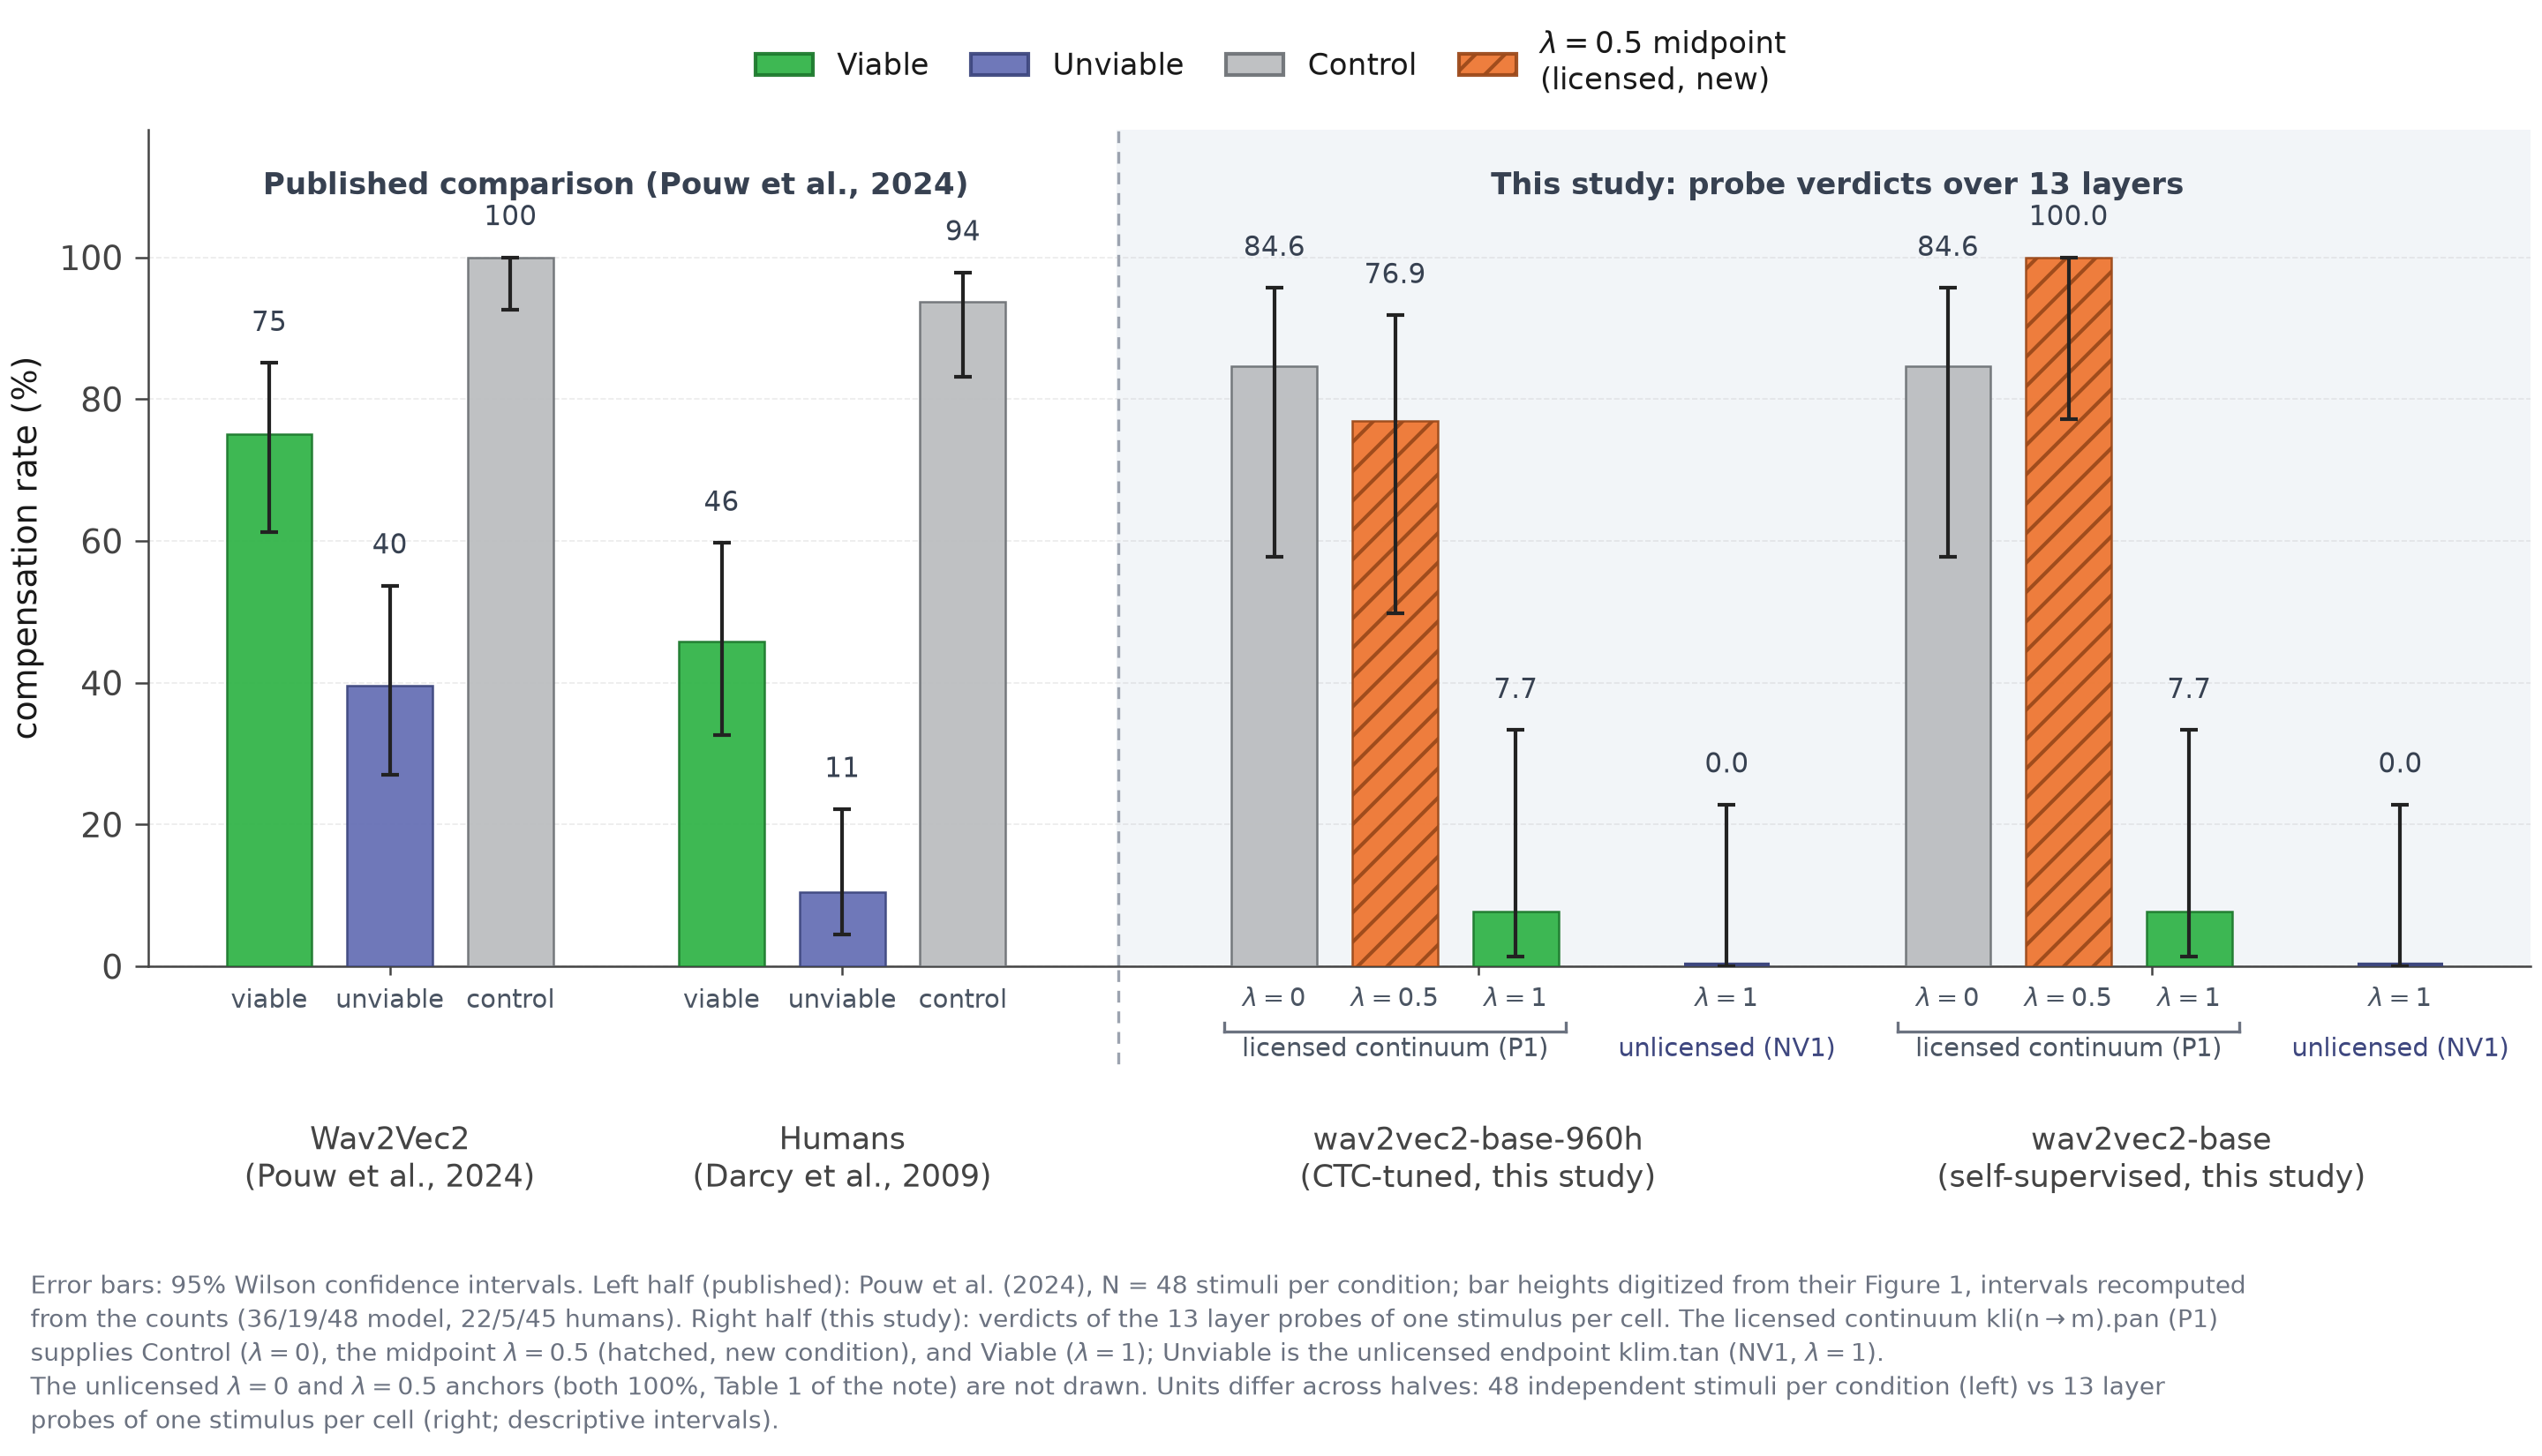
\includegraphics[width=\textwidth]{figN2_pouw_schema_reproduction.png}
\caption{The schema of Pouw et al.'s Figure~1, reproduced and
extended. Left half (published): compensation rates of the
transcription measure for Wav2Vec2 and for the human listeners of
\citet{darcy2009} in viable, unviable, and control contexts; bar
heights digitized from their figure ($k/48$ estimated as 36/19/48
and 22/5/45 out of 48), Wilson intervals recomputed. Right half
(this study): the pooled probe-verdict rates of
Table~\ref{tab:rates}, with the bars of each listener assembled
along the licensed cluster continuum---Control = $\lam=0$ (canonical
clusters \sampa{klinpan}, \sampa{minbot}, \sampa{Tinpakit}), the
gestural midpoint $\lam=0.5$ (hatched, the condition the published
design cannot express), Viable = licensed $\lam=1$ (target-assimilated
clusters)---and the Unviable bar (unlicensed $\lam=1$,
\sampa{klintan}/\sampa{klinkan}/\sampa{mingot}) one step outside the
continuum bracket. The viable bars of the right half sit at or below
their unlicensed counterparts---the inverted divergence from the
published comparison. Units differ across the halves: 48 independent
stimuli per condition on the left, 39 layer-probe verdicts per cell
on the right (descriptive intervals; Section~\ref{sec:caveats}).}
\label{fig:pouwrepro}

\end{figure}

% =====================================================================
\section{A focused reproduction attempt: $\lam=0.75$ production}
\label{sec:repro075}

Section~\ref{sec:rates} locates the action at $\lam=1$: the licensed
dip of the CTC-tuned listener. The stimuli of the published comparison
were produced by a human speaker, and natural assimilation is
characteristically partial: the coronal gesture is reduced rather than
replaced. The experiment of this section therefore tests the
intermediate regime along two axes at once. First, the production
degree is set to $\lam=0.75$: three quarters of the way along the
target rotation, a strong but incomplete assimilation whose C1
gesture aims at the C2 place with the lips recruited in proportion
(LD at the C1 target point: $0.16$\,cm against $0.00$ at $\lam=1$
and $0.61$ open---three quarters closed, not the full constriction). Second,
the stimulus base is widened from one licensed and one unlicensed
carrier frame to three of each,
so that the licensed--unlicensed contrast is no longer a contrast of
single sentences: licensed frames ``clean pan'', ``mean boat'', and
``thin packet'' (\sampa{klinpan}, \sampa{minbot}, \sampa{Tinpakit};
n$\rightarrow$m before the labials /p/, /b/, /p/) against unlicensed
frames ``clean tan'', ``clean can'', and ``mean goat''
(\sampa{klintan}, \sampa{klinkan}, \sampa{mingot}; n$\rightarrow$N
before the non-labials /t/, /k/, /g/).

The three conditions now map one-to-one onto Pouw et al.'s
Figure~1. \emph{Control} is the canonical production $\lam=0$ of all
six frames (6 stimuli); \emph{Viable} is the $\lam=0.75$ production of
the three licensed frames (3 stimuli); \emph{Unviable} is the
$\lam=0.75$ production of the three unlicensed frames (3 stimuli); the
$\lam=1$ endpoints of the same six frames are retained as a
production-degree reference. The reuse discipline is now structural
rather than incremental: every cell of this section, of
Section~\ref{sec:repro0625}, and of the anchor table of
Section~\ref{sec:rates} is a slice of one 54-item campaign---six
frames $\times$ nine degrees, synthesized under the four v1.2.0
run-time guarantees (all held, 54/54), passed once through both
encoders, and read once by the unchanged probe instrument---so the
blocks of this kit re-derive one another's shared cells by
construction (asserted: maximum $|{\Delta}P(\mathrm{n})| = 0$ between
blocks) and the only degrees that could in principle differ across
sections cannot. The dotted citation tier of the earlier kits is
retained as a reference block only: the distance between the cluster
endpoints and the dotted endpoints is large (maximum
$|{\Delta}P(\mathrm{n})| = 0.86$ CTC, $0.81$ self-supervised, pooled
over the twelve frames' canon and assimilated dotted forms), which is
the quantitative statement that the tautosyllabic cluster and the C.C
split are different gestures---reported as a coarticulation distance,
not an error, and the reason no endpoint cross-check against the
dotted tier is meaningful under the revised semantics.

Table~\ref{tab:lam075} and Figure~\ref{fig:repro075} give the
result, and the intermediate degree does what an intermediate degree
should: it moves every cell of the design to the high side of its
$\lam=1$ value. The viable rate stands at 79.5\% (CTC-tuned) and
100.0\% (self-supervised)---the latter above every published cell
(46\% humans, 75\% model)---and the unviable rates at 89.7\% and
97.4\%, far above the published unviable band of 11--40\%. The
controls are the coarticulated cluster baselines of
Section~\ref{sec:rates}: 64.1\% and 61.5\%, the CTC-tuned listener
losing 28 of 78 verdicts concentrated on the two ``min'' frames
(P2 ``mean boat'' and NV4 ``mean goat'', 15 verdicts, the lexical
/m/ drift of that onset) and on the early-layer coarticulation
reading of the ``clean pan''/``thin packet'' clusters (13 verdicts,
front-loaded at CNN--T1).

The asymmetry, however, does not follow---in either direction.
The viable--unviable difference at $\lam=0.75$ is $-10.3$ points for
the CTC-tuned listener (Newcombe hybrid-score interval $[-26.5,
+6.2]$; Fisher exact $p = .35$) and $+2.6$ points for the
self-supervised one (interval $[-6.6, +13.2]$; $p = 1.0$); the
$\lam=1$ reference differences are $-20.5$ ($[-37.3, -2.4]$) and
$-17.9$ ($[-32.7, -5.3]$)---the only two intervals that exclude
zero, and the lip recruitment has made the second one significant
(it was $-10.3$ $[-23.6, +0.6]$ with the lips blocked). Against
the published asymmetry of $+35$ points in both populations, this is
a second null result---and the per-frame breakdown shows that it is
not merely a matter of statistical power. Licensed rates at
$\lam=0.75$ range from 9/13 (P2 and P4, CTC-tuned) to 13/13 (P1,
CTC-tuned; every licensed frame, self-supervised); unlicensed rates
range from 9/13 (NV4, CTC-tuned) to 13/13 (NV1 and NV3, both
listeners). The ranges interleave completely: NV3, an
\emph{unlicensed} frame (``clean can'', n before velar /k/),
compensates at 13/13 for both listeners---as high as any licensed
frame---while P2, a licensed frame, compensates at 9/13 for the
CTC-tuned listener. The nominally negative pooled asymmetry is
carried by the unlicensed pool's \emph{clean} frames (NV1, NV3 at
13/13) against the licensed pool's ``thin packet'' and ``mean boat''
(9/13), i.e.\ by cluster coarticulation and lexical onsets, not by
licensing.

At the probability level the picture is the same. Pooling the three
frames per condition, the layer-wise mean $P(\mathrm{n})$ of the viable
and unviable conditions never differs by more than .24 (CTC-tuned,
T11: .355 viable against .590 unviable; the self-supervised maximum
is .09), and the sign of the difference is uniformly negative for
the CTC-tuned listener (deep means .403 viable against .573
unviable), near-zero for the self-supervised one (.697 against
.659). The direction is the inverted asymmetry again: it is the
licensed pool that reads slightly less /n/, at the depths where the
labial cluster context lives. Item identity---the ``min'' onsets, the
coarticulation strength of each cluster---organizes the probability
field more strongly than phonological license at every production
degree tested.

What the experiment reproduces, then, is the \emph{level} structure
of the published Figure~1 on its high side: compensation in the
assimilated conditions at or above the published band, and a strong
sensitivity to the production degree (moving the CTC-tuned viable
cell from $\lam=1$ to $\lam=0.75$ raises it by $+10.3$ points, the
self-supervised one by $+17.9$; both rise by a further $+30.8$ and
$+51.3$ from $\lam=0$ to $\lam=0.75$, the coarticulation baseline
being what it is). What it does not reproduce is the figure's
\emph{contrast} structure: compensation here tracks how the gestural
rotation and the cluster coarticulation move the representation, not
whether the context licenses the surface assimilation---and the one
significant contrast we do measure points opposite to the published
direction. In the terms of Table~\ref{tab:mapping}, both listeners
behave as signal-driven perceivers at every production degree
tested; the ingredient whose absence would explain the difference
from the published comparison is precisely the phonological
licensing sensitivity that defines compensation for coarticulation.

\begin{table}[t]
\small
\centering
\begin{tabular}{@{}lccccc@{}}
\toprule
 & Control & Viable & Unviable & Viable & Unviable \\
 & ($\lam=0$) & ($\lam\!=\!.75$) & ($\lam\!=\!.75$) & ($\lam\!=\!1$, ref) & ($\lam\!=\!1$, ref) \\
\midrule
Wav2Vec2$^{\dagger}$ & 100 & 75 & 40 & n/a & n/a \\
Humans$^{\dagger}$ & 94 & 46 & 11 & n/a & n/a \\
\addlinespace
960h (ours) & 64.1 [53.0, 74.0] & 79.5 [64.1, 89.3] & 89.7 [76.0, 95.8] & 69.2 & 89.7 \\
base (ours) & 61.5 [50.2, 71.6] & 100.0 [91.0, 100.0] & 97.4 [86.8, 99.5] & 82.1 & 100.0 \\
\bottomrule
\end{tabular}
\caption{Compensation rates (\%, verdict /n/) of the reproduction
attempt with $\lam=0.75$ as the production degree, in the layout of
Pouw et al.'s Figure~1. Control: $\lam=0$ canonical cluster pooled
over the six frames ($k/78$); Viable/Unviable (test): $\lam=0.75$
pooled over the three licensed/unlicensed frames ($k/39$); the two
rightmost columns restate the $\lam=1$ reference over the same frames.
Brackets: 95\% Wilson score intervals. $^{\dagger}$Digitized from the
published figure ($k/48 = 36/19/48$ for the model and 22/5/45 for the
humans of \citealp{darcy2009}); the published design has no
production-degree analogue. Denominators: 78 and 39 (stimuli $\times$ 13
layer probes) against the published 48 independent stimuli per
condition.}
\label{tab:lam075}
\end{table}

\begin{figure}[t]
\centering
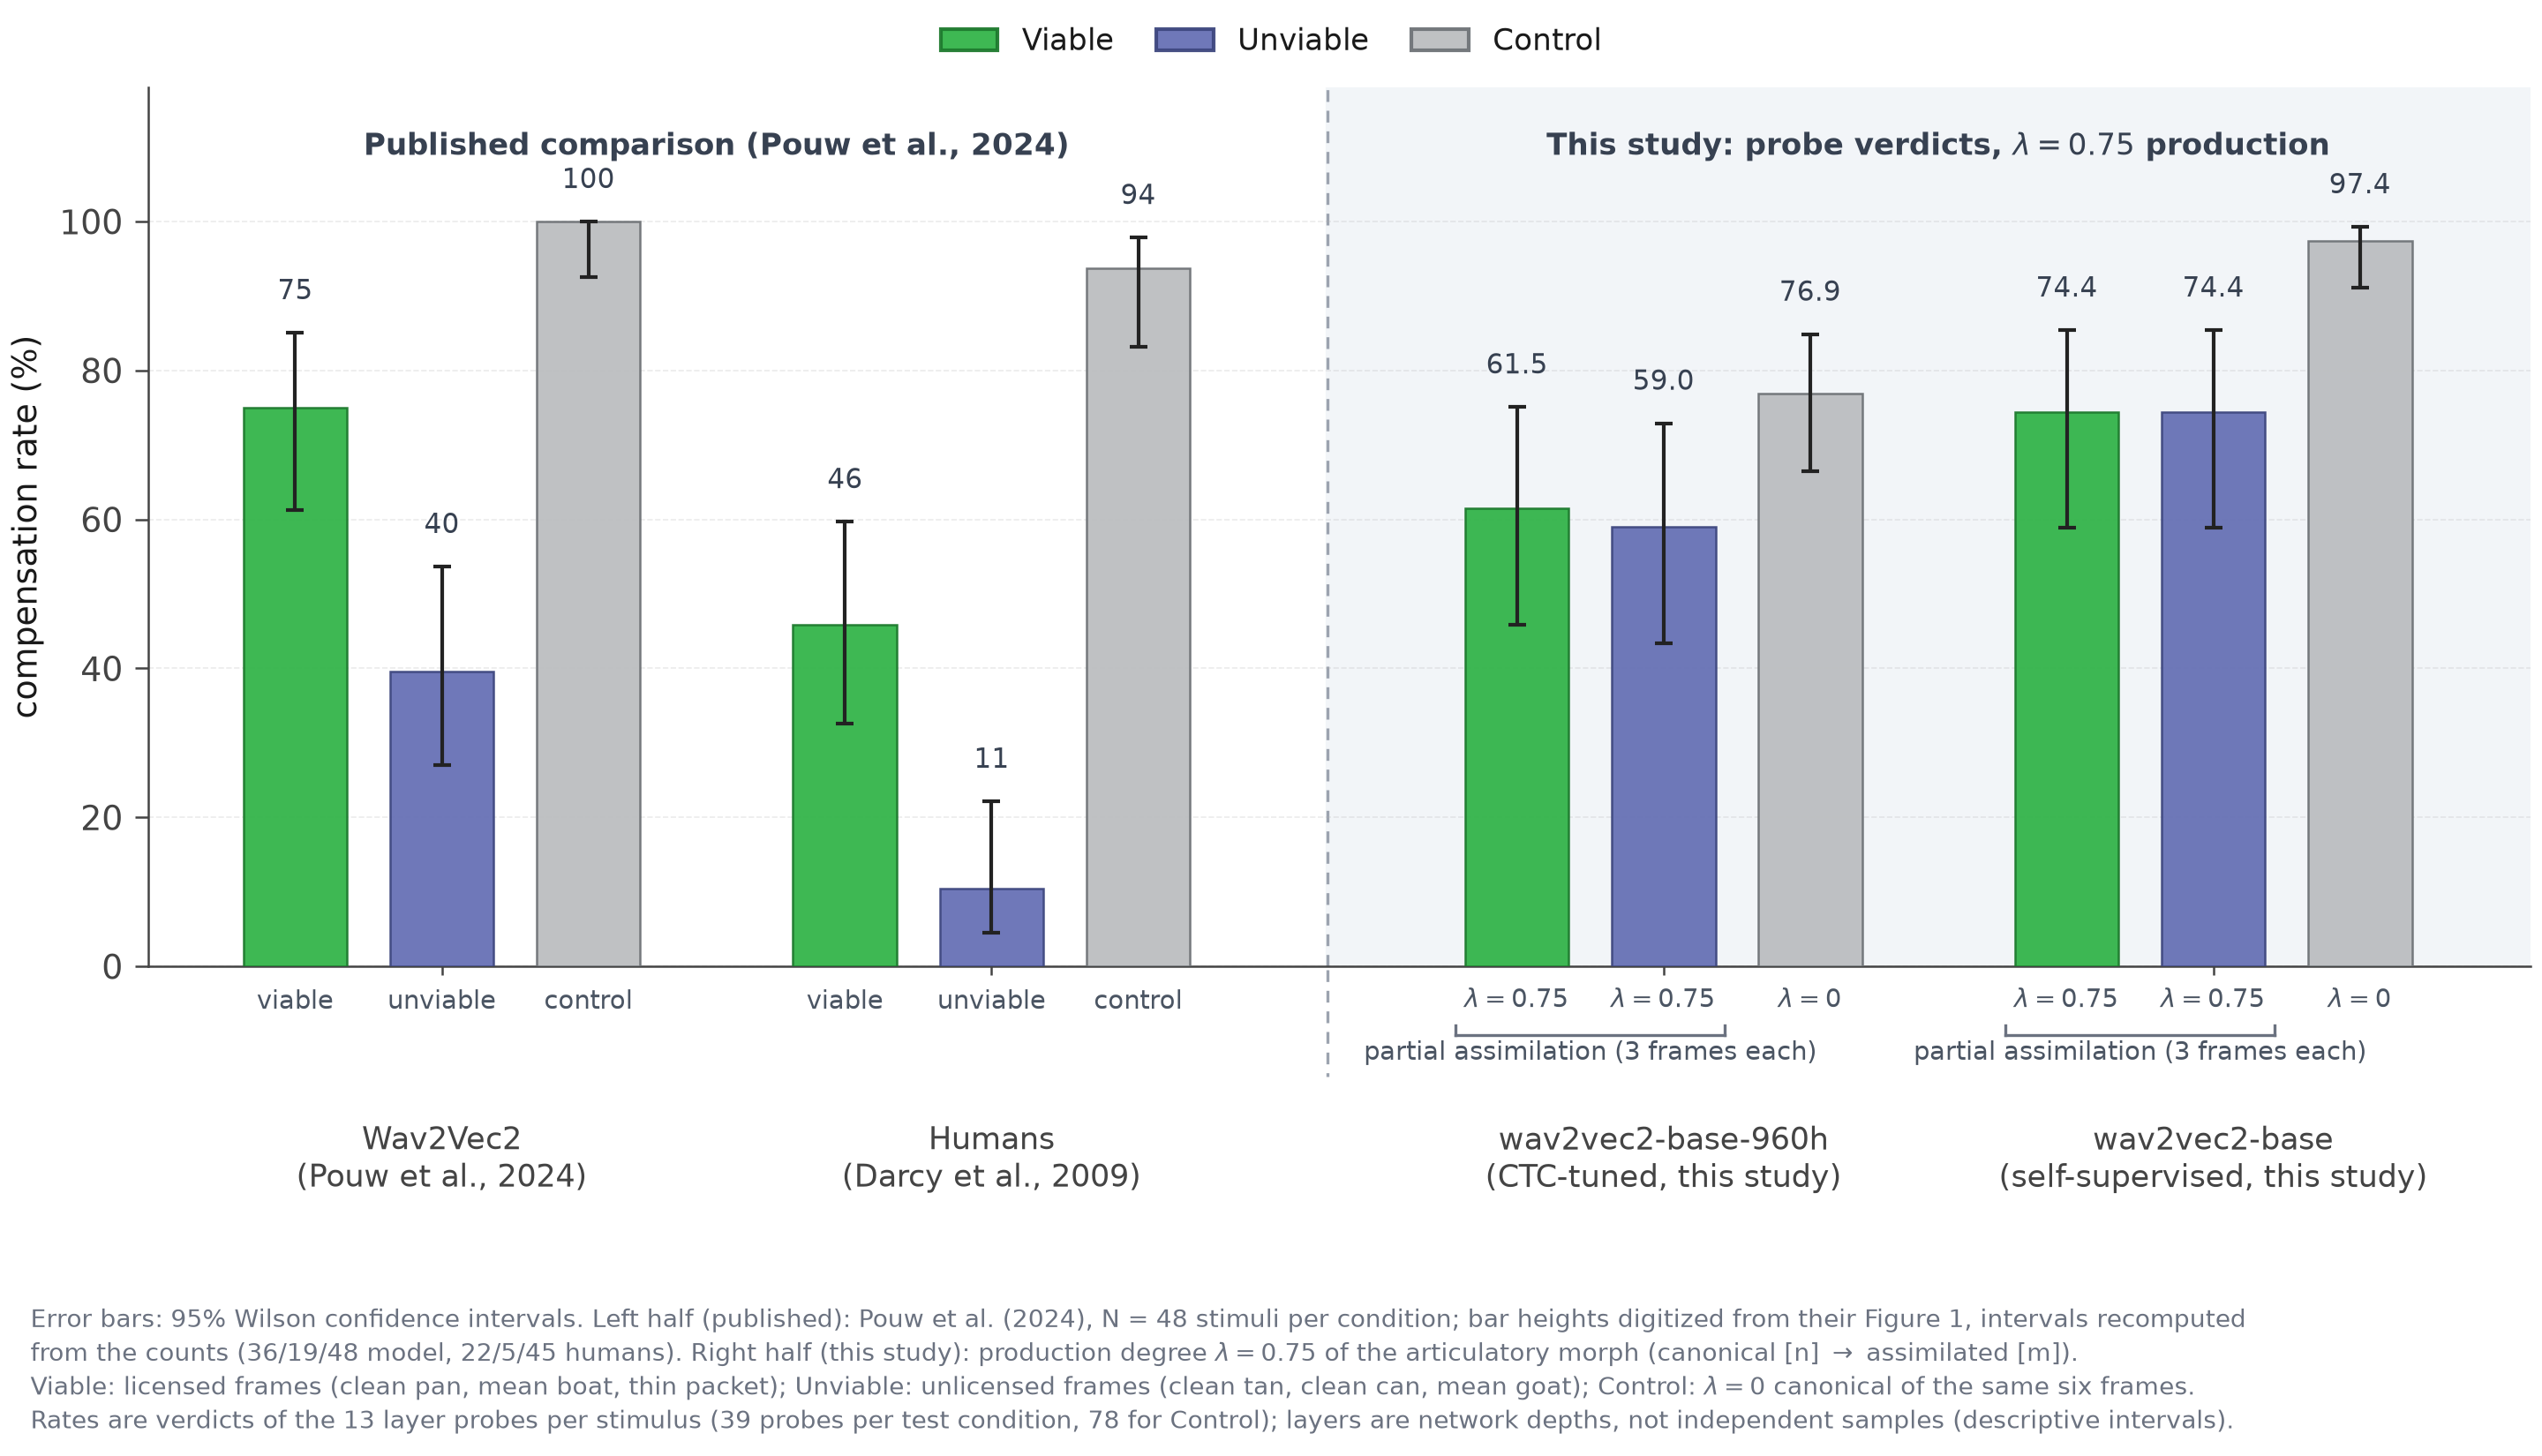
\includegraphics[width=\textwidth]{figN3_pouw_reproduction_lam075.png}
\caption{The schema of Pouw et al.'s Figure~1 with the reproduction
attempt of Section~\ref{sec:repro075}. Left half: the published
comparison (bar heights digitized, intervals recomputed), as in
Figure~\ref{fig:pouwrepro}. Right half: the two listeners of this
study under the $\lam=0.75$ production protocol, in the published
condition order so that every bar aligns with its published
counterpart---Viable: licensed frames \emph{clean pan}, \emph{mean
boat}, \emph{thin packet}; Unviable: unlicensed frames \emph{clean
tan}, \emph{clean can}, \emph{mean goat}; Control: $\lam=0$ canonical
cluster production of the same six frames. The production-degree
manipulation reproduces the published levels on the high side (79.5\%
and 100.0\% viable against 46--75\% published; 89.7\% and 97.4\%
unviable against 11--40\%) but not the viable--unviable
asymmetry: $-10.3$ points $[-26.5, +6.2]$ (CTC-tuned) and $+2.6$
$[-6.6, +13.2]$ (self-supervised) against $+35$ points in both
published populations. Units: 48 independent stimuli per condition
(left) against (stimuli $\times$ 13 layer probes)---39 per test
condition, 78 per control---on the right (descriptive intervals;
Section~\ref{sec:caveats}).}
\label{fig:repro075}
\end{figure}

% =====================================================================
\section{A second production degree: $\lam=0.625$}
\label{sec:repro0625}

The $\lam=0.75$ attempt locates the failure of the reproduction
precisely: the production degree controls the compensation
\emph{level}, and nothing in the comparison so far recovers the
published \emph{contrast}. A licensing modulation, if these listeners
harbor one, has the best chance of showing where compensation is high
in \emph{both} frame classes---so that a context-driven separation
has room to operate---and where the residual alveolar cue is still
strong. Both considerations point away from $\lam=1$ and towards the
canonical end of the continuum. This section therefore re-runs the
identical six-frame protocol with $\lam=0.625$---five eighths of the
way from [n] to [m]---as the production degree. Nothing else
changes: the same three licensed and three unlicensed frames, the
same 18 canonical training sentences, the same 13 layer probes per
stimulus, the same three-condition mapping onto Pouw et al.'s
Figure~1.

The reuse discipline remains structural: the $\lam=0.625$ cells are
slices of the same 54-item campaign as every other degree, measured by
the same single probing run (the block-to-block identity is asserted
at 0.000000, cell by cell), so the new degree is measured against a
background that is, by construction, the same experiment. The
controls of Table~\ref{tab:lam0625} are therefore identical to those
of Table~\ref{tab:lam075} by construction rather than by coincidence,
and---unlike every earlier edition of this note---so are the
$\lam=0.75$ and $\lam=1$ reference columns.

Table~\ref{tab:lam0625} and Figure~\ref{fig:repro0625} give the
three-condition result. The levels sit at or above their $\lam=0.75$
values: the viable rates at 79.5\% (CTC-tuned) and 100\%
(self-supervised), the unviable rates at 89.7\% and 94.9\%. The
self-supervised listener now exceeds every published cell (100\%
viable against 46--75\%; 94.9\% unviable against 11--40\%): at this
degree the listeners recover the underlying /n/ on four fifths or
more of the probes irrespective of context---they over-compensate
everywhere, exactly as the gestural reading of the revised continuum
predicts (the mid-continuum is where the rotation has cleaned the
coarticulated baseline without yet arming the late labial reading).
The controls are unchanged by construction (64.1\% and 61.5\%).

The asymmetry remains absent, and its sign structure is now
diagnostic. The viable--unviable difference at $\lam=0.625$ is
$-7.7$ points (Newcombe interval $[-23.7, +8.4]$; Fisher exact
$p = .52$) for the CTC-tuned listener and $+5.1$ points
($[-4.6, +16.9]$; $p = .49$) for the self-supervised one---nominally
of opposite sign, against $+35$ points in both published populations.
Across the three degrees now tested the differences read $-20.5$,
$-7.7$, $-10.3$ (CTC-tuned, from $\lam=1$ down) and $-17.9$, $+2.6$,
$+5.1$ (self-supervised): nothing positive before the moderate
degrees, two intervals excluding zero (the $\lam=1$ licensed dips of
both listeners), and nothing that resembles the published gradient. The per-frame breakdown shows the same
interleaving as at $\lam=0.75$---the unlicensed ``clean can''
compensates at 13/13 for both listeners, as high as any licensed
frame, while the licensed ``mean boat'' sits at 9/13 for the
CTC-tuned listener---and the nominal differences are carried by the
same item effects that organize the $\lam=0$ baseline.

Figure~\ref{fig:dose} assembles the dose-response over all nine
degrees of the campaign grid---the v2.1 note could plot four, the
single-run design makes all nine available at no cost. Three
regularities are visible at a glance. First, every track \emph{rises}
from $\lam=0$: the canonical cluster baseline is the low point of
each curve, and the first eighth of the target rotation already
cleans most of the coarticulation reading (CTC-tuned viable: 48.7\%
at $\lam=0$, 79.5\% at $\lam=0.125$). Second, the mid-continuum is a
plateau (roughly 72--80\% for the CTC-tuned licensed track, 84--95\%
unlicensed, ceiling throughout for the self-supervised listener):
this is the regime the published design would call partial
assimilation, and it is where the listeners are most canonical.
Third, the licensed track of the CTC-tuned listener dips at the
endpoint (74.4\% at $\lam=0.875$ down to 69.2\% at $\lam=1$) while
its unlicensed track does not---the $\lam=1$ licensed dip again,
visible here as the only end-of-continuum descent in the figure; the
self-supervised licensed track, ceiling-bound through the
mid-continuum, now descends at the endpoint too (89.7\% at
$\lam=0.875$ to 82.1\% at $\lam=1$)---the bilateral dip.
The unlicensed track sits above the licensed one at every degree for
the CTC-tuned listener (largest gap 30.8 points at $\lam=0$, the
coarticulation asymmetry of the canonical clusters) and at most
degrees for the self-supervised one. At the probability level the
$\lam=0.75$ pattern repeats: the layer-wise mean
$P(\mathrm{n})$ difference (viable minus unviable) reaches $-.312$
at T11 for the CTC-tuned listener (deep means .367 against .612;
$-.282$ at T12: .440 against .722) and never exceeds $.170$ in
absolute value for the self-supervised one (.769 against .651,
the viable side higher at every level but T8).

Nine production degrees now bracket the response function, and the
conclusion of Section~\ref{sec:repro075} survives its strongest
test intact. The experiments reproduce---and overshoot---the
published \emph{levels}: viable cells at or above the published band
from $\lam=0.125$ onward, unviable cells far above it everywhere.
They do not reproduce the published \emph{contrast} at any degree:
the viable--unviable difference is negative or null wherever it is
measured (the licensed pool starts lower, at the coarticulated
baseline, and ends lower, at the letter-supervised labial reading),
and the item identity of the carrier frames organizes the
probability field more strongly than phonological license at every
point of the continuum tested.

\begin{table}[t]
\small
\centering
\begin{tabular}{@{}lccccc@{}}
\toprule
 & Control & Viable & Unviable & Viable & Unviable \\
 & ($\lam=0$) & ($\lam\!=\!.625$) & ($\lam\!=\!.625$) & ($\lam\!=\!.75$, ref) & ($\lam\!=\!.75$, ref) \\
\midrule
Wav2Vec2$^{\dagger}$ & 100 & 75 & 40 & n/a & n/a \\
Humans$^{\dagger}$ & 94 & 46 & 11 & n/a & n/a \\
\addlinespace
960h (ours) & 64.1 [53.0, 74.0] & 79.5 [64.1, 89.3] & 89.7 [76.0, 95.8] & 79.5 & 89.7 \\
base (ours) & 61.5 [50.2, 71.6] & 100.0 [91.0, 100.0] & 94.9 [83.1, 98.6] & 97.4 & 97.4 \\
\bottomrule
\end{tabular}
\caption{Compensation rates (\%, verdict /n/) of the second
production degree, $\lam=0.625$, in the layout of Pouw et al.'s
Figure~1. Control: $\lam=0$ canonical production pooled over the six
frames ($k/78$); Viable/Unviable (test): $\lam=0.625$ pooled over
the three licensed/unlicensed frames ($k/39$); the two rightmost
columns restate the $\lam=0.75$ test of Section~\ref{sec:repro075}
over the same frames (its $\lam=1$ reference rates were 69.2/89.7 and
82.1/100.0). Brackets: 95\% Wilson score intervals.
$^{\dagger}$Digitized from the published figure ($k/48 = 36/19/48$
for the model and 22/5/45 for the humans of \citealp{darcy2009}).
Denominators: 78 and 39 (stimuli $\times$ 13 layer probes) against
the published 48 independent stimuli per condition.}
\label{tab:lam0625}
\end{table}

\begin{figure}[t]
\centering
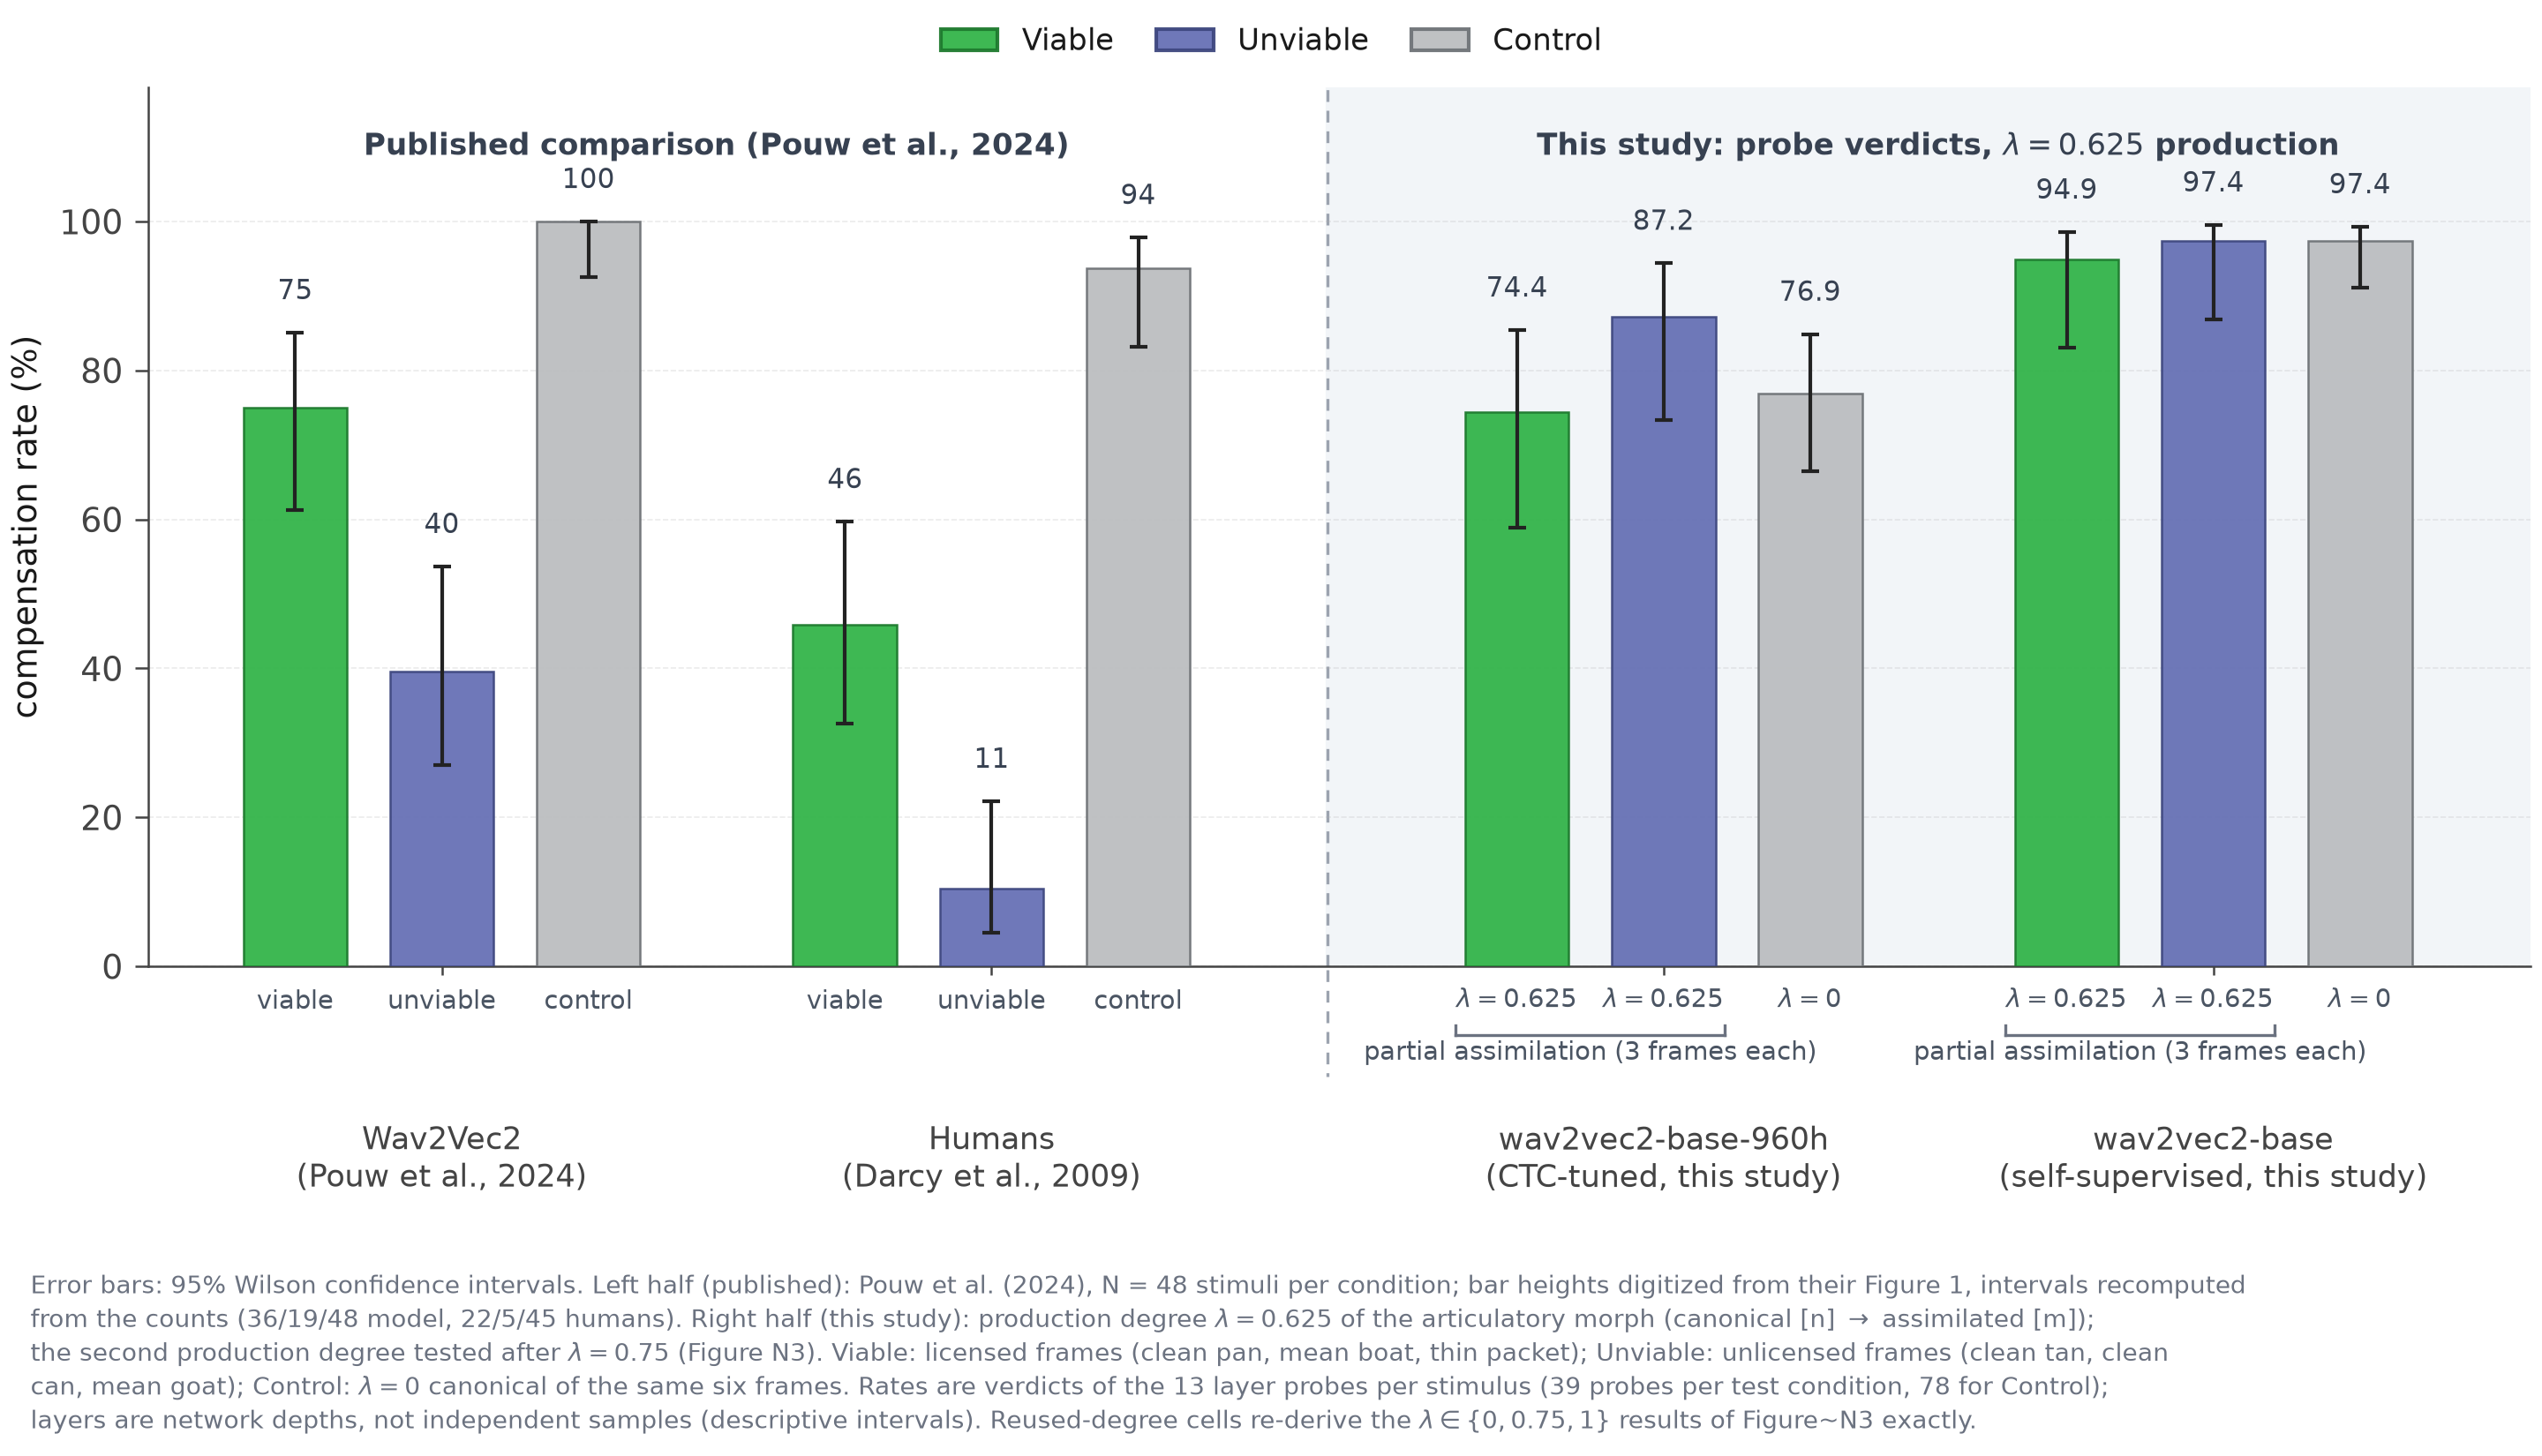
\includegraphics[width=\textwidth]{figN4_pouw_reproduction_lam0625.png}
\caption{The schema of Pouw et al.'s Figure~1 with the
$\lam=0.625$ production of Section~\ref{sec:repro0625}, layout as
Figure~\ref{fig:repro075}. Left half: the published comparison (bar
heights digitized, intervals recomputed). Right half: the two
listeners of this study under the $\lam=0.625$ production
protocol---Viable: licensed frames \emph{clean pan}, \emph{mean
boat}, \emph{thin packet}; Unviable: unlicensed frames \emph{clean
tan}, \emph{clean can}, \emph{mean goat}; Control: $\lam=0$ canonical
cluster production of the same six frames. The second production
degree reproduces and overshoots the published viable levels (79.5\%
and 100\% against 46--75\% published) with unviable cells far
above the published band (89.7\% and 94.9\% against 11--40\%), but
not the viable--unviable asymmetry: $-10.3$ points $[-26.5, +6.2]$
(CTC-tuned) and $+5.1$ $[-4.6, +16.9]$ (self-supervised) against
$+35$ points in both published populations. Units: 48 independent
stimuli per condition (left) against (stimuli $\times$ 13 layer
probes)---39 per test condition, 78 per control---on the right
(descriptive intervals; Section~\ref{sec:caveats}).}
\label{fig:repro0625}
\end{figure}

\begin{figure}[t]
\centering
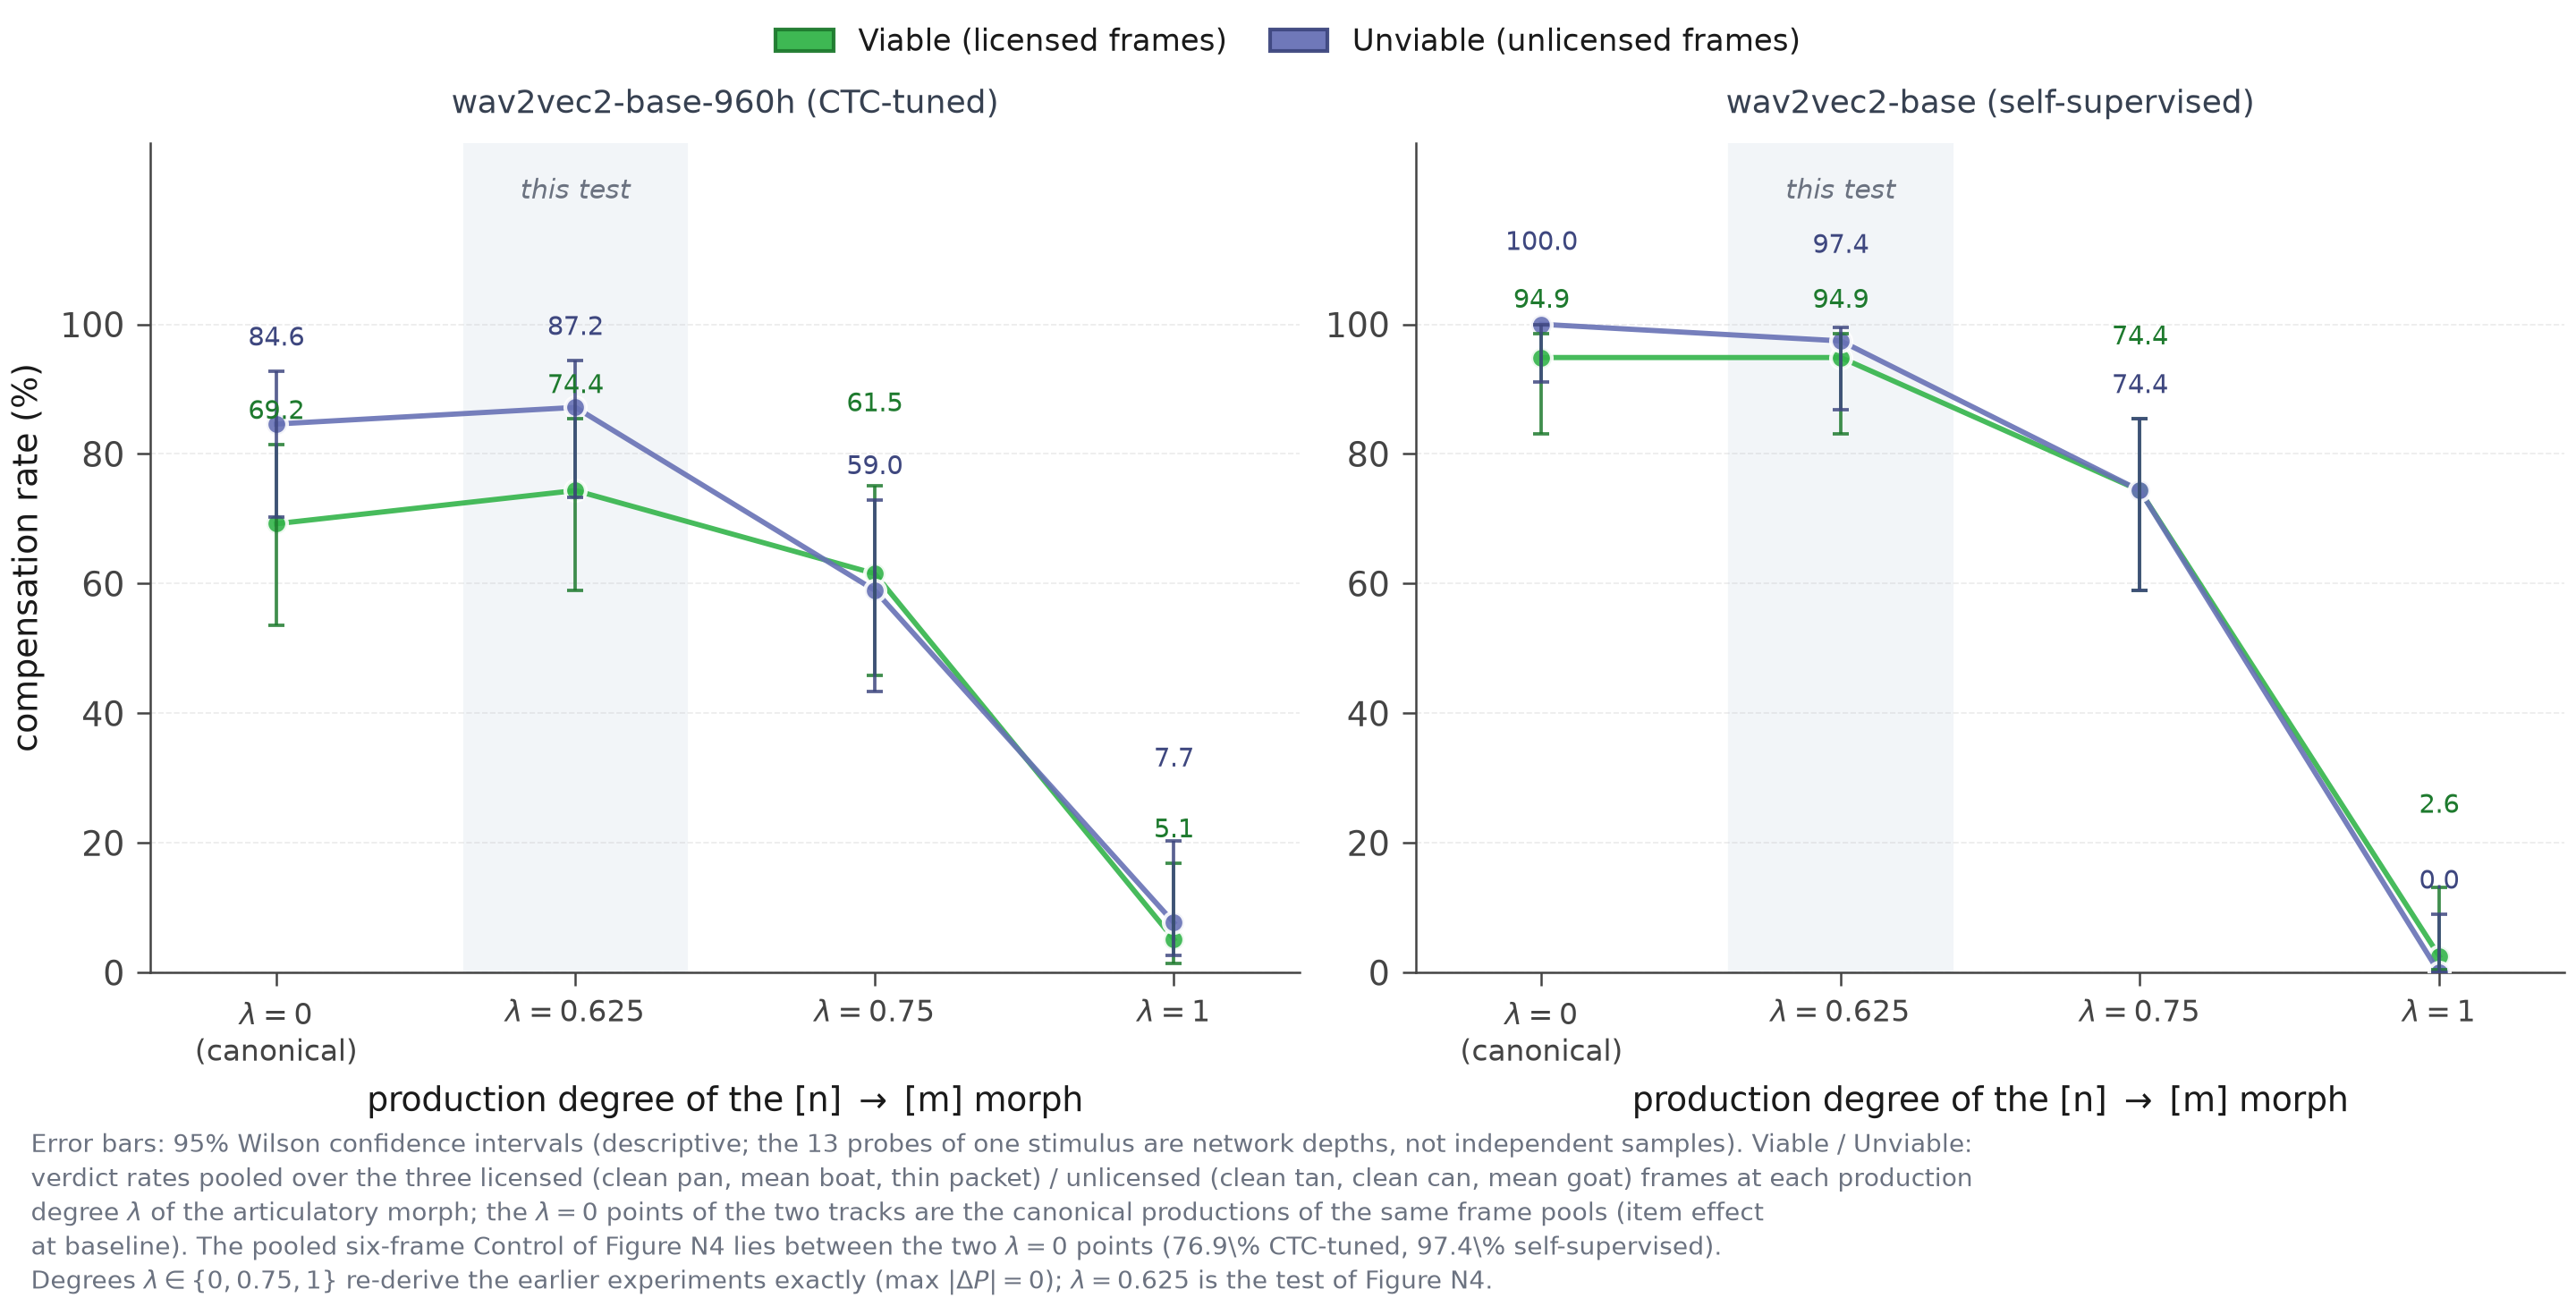
\includegraphics[width=\textwidth]{figN5_production_dose_response.png}
\caption{The production-degree dose-response of the six-frame
protocol: compensation rate of the licensed (viable, green) and
unlicensed (unviable, indigo) frame pools at each of the nine
production degrees $\lam$ of the campaign grid, per listener; error
bars are 95\% Wilson intervals. The $\lam=0$ points of the two
tracks are the canonical cluster productions of the same frame pools
(the pooled six-frame Control of Figure~\ref{fig:repro0625} lies
between them: 64.1\% CTC-tuned, 61.5\% self-supervised); all nine
degrees come from the single 54-item continuum probing run. Every
track rises from its $\lam=0$ baseline (the coarticulated cluster
canonical is the low point) and plateaus through the mid-continuum;
the licensed tracks descend at the endpoint (74.4\% at $\lam=0.875$
to 69.2\% at $\lam=1$ for the CTC-tuned listener, 89.7\% to 82.1\%
for the self-supervised one)---the late-layer labial reading, now
bilateral. The unlicensed track sits above the licensed one at every
degree for the CTC-tuned listener (largest gap 30.8 points at
$\lam=0$, the coarticulation asymmetry of the canonical clusters).
No licensing asymmetry in the published direction appears at any
degree tested.}
\label{fig:dose}
\end{figure}


% =====================================================================
\section{Crossing with the natural stimuli of the released archive}
\label{sec:lexamb}

Every experiment in this note so far probes our own VocalTractLab
synthesis, and the null licensing asymmetry that survives three
production degrees could in principle be a property of the synthetic
domain rather than of the listeners. The cleanest control would be
the natural recordings behind the published comparison itself. The
stimuli of \citet{darcy2009} that Pouw et al.'s Figure~1 replays are
not publicly available---their repository
(\path{github.com/CharlottePouw/assimilation}) carries the analysis
notebooks and scripts only, and the private \path{stimA} Drive
folder those notebooks reference is not shared. What the authors did
release, through the Google-Drive archive linked in the same
notebook, is their own natural re-recording of the Gaskell and
Marslen-Wilson \citeyearpar{gmw2001} lexical-ambiguity materials:
86 sentences recorded to be directly comparable to the Darcy
recordings (General American, deliberately pronounced assimilated
surface forms, footnote~2 of the published article). That archive is
the natural-stimulus set this section crosses with.

Decoding the archive is part of the experiment, and its structure
came out of the alignment itself. Each of the 43 numbered items is a
biasing context sentence followed by a target sentence containing
the assimilated surface word in a \emph{viable} context (``It's best
to start the day with a burst of activity. I think a quick ru[m]
picks you up.''); 38 items are exactly the Appendix~C set of the
published article ($N=38$ per condition in their Experiments~2 and~3),
and 5 items (numbers 18, 19, 20, 42, 43) are the velar-nasal
surfaces (\emph{ban}$\rightarrow$ba[ng], \emph{ran}$\rightarrow$ran[g],
\emph{bun}$\rightarrow$bu[ng], \emph{pan}$\rightarrow$pa[ng],
\emph{fan}$\rightarrow$fa[ng]) that the authors excluded because
their transcription measure cannot score [ŋ]: wav2vec2 writes the
velar nasal as two characters, $\langle$n$\rangle$$\langle$g$\rangle$.
Each item exists in two recorded passes (\path{\_1}/\path{\_2}); the
passes are two takes of the same speaker rather than the male
replication speaker of their Appendix~A---median f0 165.3 vs 163.3 Hz
across the 43 pairs, LPC spectral envelopes with an F1 ratio of
0.996, and identical pitch floors---so the crossing reports pooled
and per-pass rates. The unviable companion sentences of the original
design (``a quick ru[m] does you good'') were not part of the
release.

Two measures are run on these 86 sentences, both aligned by the CTC
greedy stream of the 960h listener: the target word is located
through its expected spellings (with a follower-word anchor as
fallback), and the assimilated consonant is the last \{m, n\}
character run of that word (for the velar items, the last \{n\} run
extended through an adjacent \{g\}). The \emph{transcription measure}
follows Pouw et al.\ exactly: compensation is scored when the
transcribed word is the underlying spelling rather than the surface
spelling, decided by nearest Levenshtein distance. The \emph{probe
measure} is this kit's own instrument: the same 13 layer probes,
trained on the same 18 canonical synthetic training sentences as
every experiment above, applied to the window mean of the hidden
states over the aligned consonant frames ($\pm2$ frames, $\approx$
100 ms, with margins 0 and 1 as sensitivity checks; the verdict is
stable across all three margins for every cell reported below). The
probes classify \{n, m, ŋ\}, so the measure applies to the 10
$n\!\rightarrow\!$m items of the analyzed set ($20$ stimuli) and,
exploratorily, to the 5 velar items ($10$ stimuli) that the
published design could not score.

\begin{table}[t]
\centering\small
\begin{tabularx}{\textwidth}{lYYr}
\toprule
Cell & $k/n$ & Rate [95\% Wilson] & Source \\
\midrule
\multicolumn{4}{l}{\emph{Transcription measure (wav2vec2-base-960h)}}\\
Viable, biasing --- published & 6/38 & 15.8 [7.4, 30.4] &
their Fig.~2, digitized \\
Viable, biasing --- this re-run & 11/76 & 14.5 [8.3, 24.1] &
released archive \\
\quad pass A / pass B & 6/38, 5/38 & 15.8, 13.2 & same \\
Unviable --- published & 0/38 & 0.0 [0.0, 9.2] &
their Fig.~2, digitized \\
Unviable --- this re-run & --- & not in the archive & --- \\
\quad $n\!\rightarrow\!$m subset / stops subset & 2/20, 9/56 &
10.0, 16.1 & same \\
\midrule
\multicolumn{4}{l}{\emph{Probe measure, natural [m] frames ($n=20$)}}\\
CTC-tuned, T12 verdicts & 0/20 & 0.0 [0.0, 16.1] & this study \\
Self-supervised, T12 verdicts & 17/20 & 85.0 [64.0, 94.8] &
this study \\
\quad pooled over 13 layers & 6/260, 65/260 & 2.3, 25.0 & same \\
\midrule
\multicolumn{4}{l}{\emph{Probe measure, natural [ŋ] frames
(exploratory, $n=10$)}}\\
CTC-tuned, T12 verdicts & 0/10 & 0.0 [0.0, 27.8] & this study \\
Self-supervised, T12 verdicts & 9/10 & 90.0 [59.6, 98.2] &
this study \\
\bottomrule
\end{tabularx}
\caption{The natural-stimulus crossing. The transcription measure
replicates the published level on the same materials (14.5\% against
a digitized 15.8\%); the probe measure dissociates the two listeners
on the natural assimilated frames. The velar-nasal items are the
ones the published measure excluded; the probe classes cover them.
Denominators: 76 sentences (38 items $\times$ 2 passes) for the
transcription measure; 20 and 10 stimuli for the probe cells, whose
layer-pooled denominators (260, 130) treat network depth as the
unit, as elsewhere in this note.}
\label{tab:lexamb}
\end{table}

Table~\ref{tab:lexamb} and Figure~\ref{fig:lexamb} give the result.
The transcription measure first: our re-run of the released archive
scores 11/76 (14.5\%, Wilson [8.3, 24.1]) compensations on the
viable natural stimuli, with the two passes in close agreement (6/38
and 5/38). The published biasing-context bars of their Figure~2,
digitized from the PDF at 2.95 px per percentage point against the
tick calibration, read 6/38 (15.8\%) viable and 0/38 unviable---the
re-run lands within a point of the published value on the same
materials, which is as direct a replication of the published
behavioral level as the released archive allows. The same ASR head
on our synthetic continuum returns nothing scorable at all: all 24
transcriptions (six frames $\times$ four degrees) are non-lexical
(``give yo panmen'', ``la lepo''), which documents, from the
crossing side, why this kit measures probes rather than
transcriptions on the synthesis---and why the note's published
comparisons on the synthetic side are probe-based.

The probe measure then delivers the crossing. On the natural
assimilated [m] frames, the self-supervised listener performs the
deep-layer shift that the synthetic experiments attribute to it: the
verdict rate for the underlying /n/ rises from 0/20 at the CNN
through 12/20 at T8 to 17/20 at T12 (85\%, [64.0, 94.8]; mean
$P(\mathrm{n})=0.69$), and the layer-pooled rate is 25.0\% against
the CTC-tuned listener's 2.3\%. The CTC-tuned listener, by contrast,
does not shift: 0/20 verdicts at T12, at every window margin, with
mean $P(\mathrm{n})$ never exceeding 0.26 (T1) and the surface mass
dominant at depth---whereas on the synthetic licensed stimuli of the
moderate degrees its representational compensation was the majority
pattern (61.5\% pooled at $\lam=0.75$, front-loaded through
T2--T5). The two listeners' deep behavior on natural assimilation is
thus a clean supervision contrast---17/20 against 0/20 at
T12---that the synthetic side had only suggested (at $\lam=0.625$,
3/3 against 1/3 licensed frames at T12). The shapes differ as well:
the self-supervised listener's natural profile rises monotonically
through depth while its synthetic moderate-degree profiles are
front-loaded and partially decay, consistent with the layer-resolved
reading of Section~\ref{sec:layers}. The exploratory velar set
tells the same story more starkly---9/10 verdicts /n/ at T12 for the
self-supervised listener against 0/10 for the CTC-tuned one---and
constitutes, to our knowledge, the first scoring of exactly the
items the published design had to drop, recovered by an instrument
(the \{n, m, ŋ\} probe) that the original transcription measure
lacks.

What the crossing establishes, then, is threefold. First, the
released natural materials reproduce the published behavioral level
through our pipeline, so the levels of the synthetic experiments can
be compared to the published ones with some confidence in the
measurement chain. Second, the probe instrument transfers across the
domain boundary: probes trained on 18 canonical synthetic sentences
deliver layer-coherent verdicts on natural recordings, and their
verdicts are not a synthesis artifact---on the natural side they
separate the two listeners exactly where the synthetic dose-response
said they should differ. Third, the supervision axis that organizes
the synthetic dose-response reappears on the natural side, sharpened:
the self-supervised stack carries the underlying nasal at depth, the
CTC-tuned stack does not. What the crossing cannot
establish is the licensing asymmetry: the released archive holds
only viable-context recordings, the natural design has no canonical
control, and the two recorded passes are two takes of one speaker.
The published viable--unviable difference on these same materials
(15.8\% against 0.0\% at the transcription level) remains the only
asymmetry measurement on natural stimuli; testing it with probes
would require the unviable recordings, which the authors have not
released.

\begin{figure}[t]
\centering
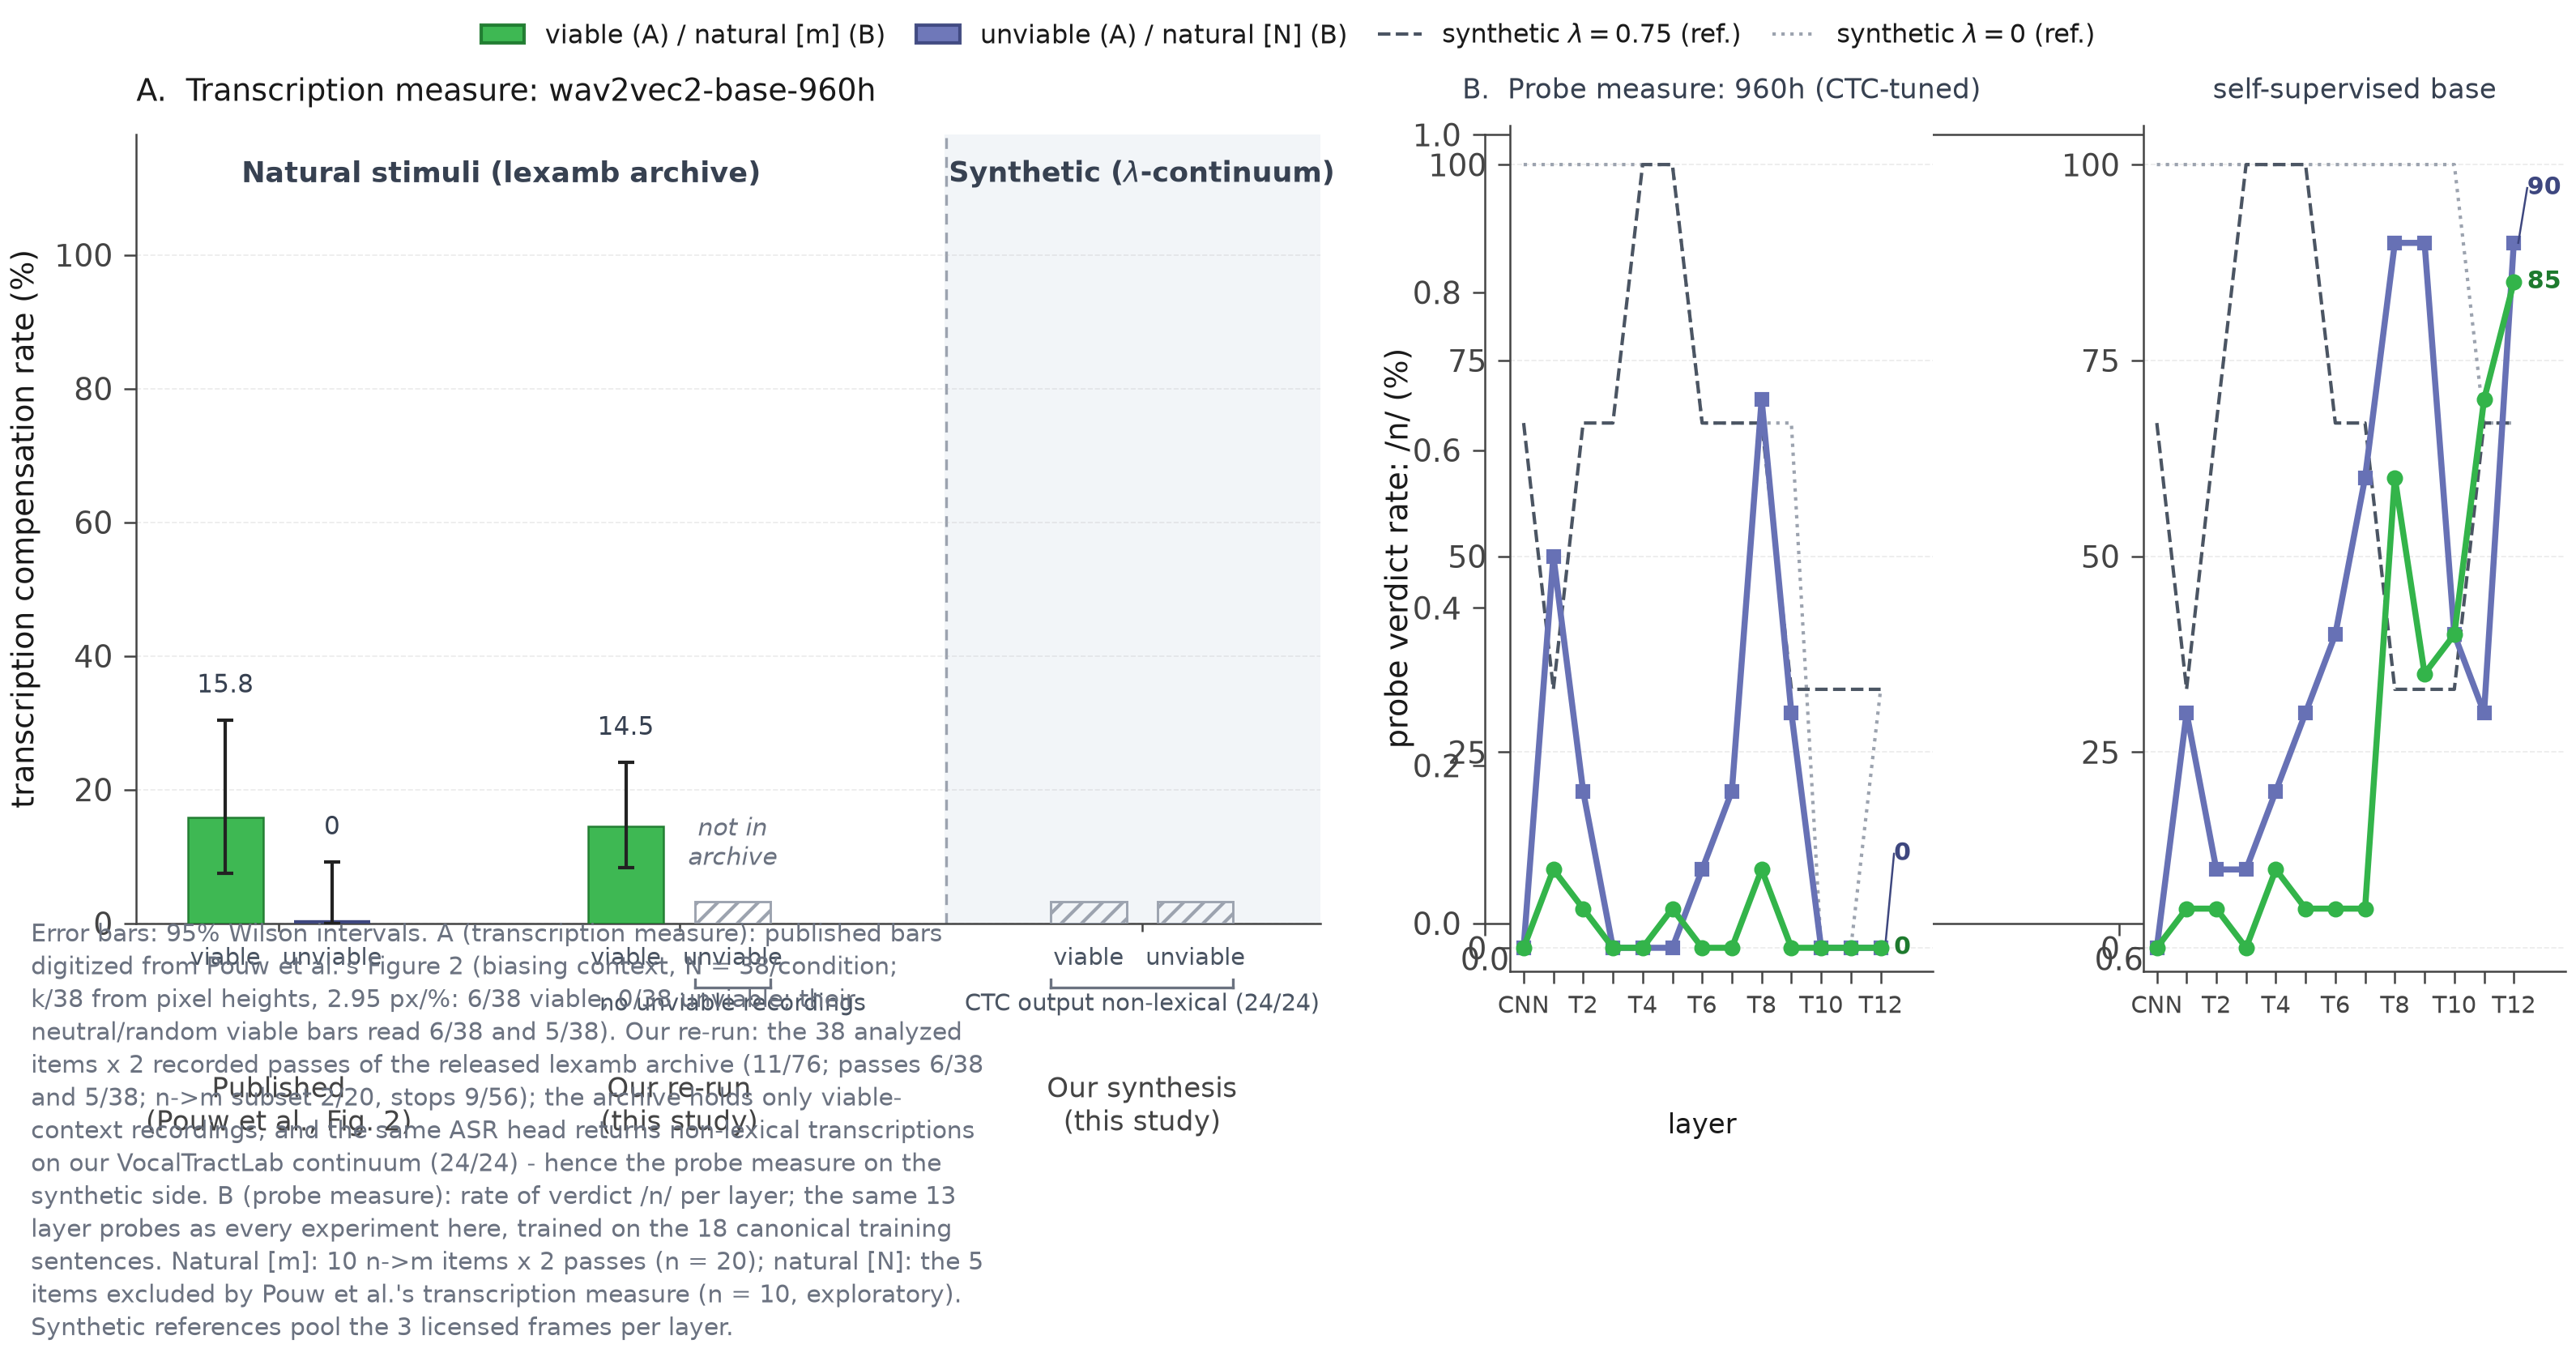
\includegraphics[width=\textwidth]{figN6_lexamb_crossing.png}
\caption{The natural-stimulus crossing. (A)~Transcription measure
(wav2vec2-base-960h): the published biasing-context bars of Pouw et
al.'s Figure~2 on the same materials (digitized, $N=38$ per
condition), our re-run of the released archive (38 analyzed items
$\times$ 2 passes), and the synthetic continuum, where the same ASR
head returns non-lexical transcriptions (24/24) so the measure is
not applicable. (B)~Probe measure: rate of verdicts for the
underlying /n/ per layer, with the same 13 synthetic-trained probes
as every experiment in this note. Natural [m] frames: the
$n\!\rightarrow\!$m items of the analyzed set ($n=20$); natural
[ŋ] frames: the five items excluded by the published transcription
measure ($n=10$, exploratory); thin references: the licensed frames
of the synthetic continuum at $\lam=0.75$ and canonical $\lam=0$.
The self-supervised listener performs the deep-layer shift on the
natural assimilated frames (0/20 at the CNN to 17/20 at T12); the
CTC-tuned listener does not (0/20 at T12, all margins).}
\label{fig:lexamb}
\end{figure}


% =====================================================================
\section{Layer-resolved probabilities}
\label{sec:layers}

Tables~\ref{tab:layers960} and \ref{tab:layersbase} report
$P(\mathrm{n})$ and $P(\mathrm{m})$ at five representative levels
(CNN, T4, T8, T11, T12) for the licensed frame P1 (\emph{clean pan},
labial C2) and the unlicensed frame NV3 (\emph{clean can}, velar C2)
of each listener---the informative contrast of the revised design;
NV1, whose rotation is nearly place-neutral, is flat by construction
and shown in the statistics blocks instead. Three observations
structure the detail. First, the phonetic layers do not track the
continuum downward at all: at T4 the probability of the underlying
/n/ never falls below $.74$ on P1 at the $\lam \geq 0.5$ anchors
(both listeners) and reaches $.95$ at NV3 $\lam=1$---the category
boundary of the earlier editions is gone. What T4 tracks instead is the \emph{coarticulation cleanup}:
the velar rotation raises $P(\mathrm{n})$ monotonically (NV3:
$.81 \rightarrow .90 \rightarrow .95$), because moving the C1 target
away from the labial-coarticulated cluster canonical moves the murmur
toward the trained /n/ centroid. The acoustic layer carries the
baseline asymmetry: at $\lam=0$ the licensed cluster reads
$/\mathrm{m}$-ish (P1: $.34/.55$ n over m for the CTC-tuned
listener) where the velar-context cluster does not (NV3:
$.50/.38$), and that difference is what the pooled control cells of
Section~\ref{sec:rates} aggregate.

\begin{table}[t]
\small
\centering
\begin{tabular}{@{}llccccc@{}}
\toprule
Context & $\lam$ & CNN & T4 & T8 & T11 & T12 \\
\midrule
Licensed (P1) & 0 & .34/.55 & .70/.27 & .44/.48 & .78/.11 & .82/.08 \\
 & 0.5 & .77/.19 & .88/.09 & .65/.28 & .78/.08 & .88/.05 \\
 & 1.0 & .41/.21 & .79/.09 & .58/.31 & .58/.09 & .71/.12 \\
\addlinespace
Unlicensed (NV3) & 0 & .50/.38 & .81/.16 & .75/.20 & .78/.12 & .89/.06 \\
 & 0.5 & .63/.28 & .90/.07 & .78/.15 & .65/.16 & .79/.15 \\
 & 1.0 & .76/.20 & .95/.03 & .84/.10 & .94/.02 & .89/.04 \\
\bottomrule
\end{tabular}
\caption{CTC-tuned \sampa{wav2vec2-base-960h}: $P(\mathrm{n})$
over $P(\mathrm{m})$ at five levels for the three anchor conditions,
licensed P1 (\emph{clean pan}, labial C2) and unlicensed NV3
(\emph{clean can}, velar C2). Under the full-selector condition the
licensed $\lam=1$ deep cells no longer cross: P1's lips now close,
and its late-layer labial reading disappears (T11: $P(\mathrm{m})
= .09$ against $.53$ with the lips blocked); the crossing lives on
P2/P4, outside this table.}
\label{tab:layers960}
\end{table}

\begin{table}[t]
\small
\centering
\begin{tabular}{@{}llccccc@{}}
\toprule
Context & $\lam$ & CNN & T4 & T8 & T11 & T12 \\
\midrule
Licensed (P1) & 0 & .35/.52 & .54/.43 & .56/.39 & .16/.66 & .18/.75 \\
 & 0.5 & .77/.18 & .91/.07 & .87/.10 & .49/.38 & .67/.25 \\
 & 1.0 & .39/.20 & .74/.12 & .76/.14 & .84/.08 & .80/.04 \\
\addlinespace
Unlicensed (NV3) & 0 & .50/.37 & .65/.32 & .70/.24 & .51/.35 & .61/.29 \\
 & 0.5 & .63/.27 & .87/.09 & .89/.07 & .51/.32 & .67/.23 \\
 & 1.0 & .75/.20 & .92/.05 & .93/.04 & .57/.24 & .73/.08 \\
\bottomrule
\end{tabular}
\caption{Self-supervised \sampa{wav2vec2-base}: $P(\mathrm{n})$
over $P(\mathrm{m})$ at five levels for the three anchor conditions,
same frames as Table~\ref{tab:layers960}. With the lips recruited,
the licensed $\lam=1$ deep cells of this listener recover fully
(T11: $P(\mathrm{n}) = .84$, against $.45$ with the lips blocked).
The $\lam=0$ licensed deep cells (T11--T12:
$P(\mathrm{n})=.16$--$.18$) are the control drift discussed in the
text.}
\label{tab:layersbase}
\end{table}

Second, the deep trajectory of the CTC-tuned listener at licensed
$\lam=1$ is the scientific heart of the note, and the full-selector
condition turns it into a clean dissociation. With the lips blocked
(v3.0) the licensed deep cells crossed: $P(\mathrm{n})$ fell to
$.42$ (T10) and $.38$ (T11) while $P(\mathrm{m})$ climbed to $.44$
and $.53$. With the lips \emph{recruited}---a true labial closure
through most of the C1 window---the crossing vanishes: P1 now runs
$.52 \rightarrow .53 \rightarrow .58 \rightarrow .71$ from T9 to
T12 with $P(\mathrm{m})$ below $.35$ throughout, thirteen of
thirteen /n/ verdicts. The late, letter-supervised labial reading
survives exactly where it already existed at $\lam=0$: on P2 and
P4 (T10--T11, $\lam=1$: $P(\mathrm{m}) = .65$--$.95$), the frames
whose cluster context---not whose lips---produced it. The unlicensed
column shows nothing of the sort: at $\lam=1$ the NV3 underlying
probability \emph{rises} with depth ($.76$ at CNN to $.94$ at T11),
and the pooled deep mean of $P(\mathrm{n})$ over T10--T12 is $.636$
unlicensed against $.232$ licensed---the inverted asymmetry again,
now at the probability level, and \emph{wider} than with the lips
blocked ($.573$ against $.360$). The self-supervised listener,
whose licensed deep cells recovered ($\lam=1$ T11: $.84$, twelve
of thirteen /n/ verdicts), shows the dip only in the pooled deep
means ($.633$ licensed against $.692$ unlicensed).

Third, the self-supervised control drift survives the change of
stimulus class: at licensed $\lam=0$, $P(\mathrm{n})$ at T11--T12
collapses to $.16$--$.18$ (the ``clean pan'' quirk, now read on the
canonical \emph{cluster} rather than the dotted citation form),
whereas one half-step into the continuum, at $\lam=0.5$, the same
cells recover to $.49$--$.67$ with unanimous /n/ verdicts. The drift
is thus a sharply local property of the canonical token rather than
a graded property of the continuum, present in both stimulus tiers,
which is also why it inflates that listener's positive deep
contrasts without disturbing the rank statistics computed over the
nine steps (Section~\ref{sec:continuum}).

% =====================================================================
\section{Continuum statistics}
\label{sec:continuum}

Figure~\ref{fig:rates}c plots the layer-wise Spearman correlation
$\rho(\lam, P(\mathrm{n}))$ on the pooled layer means of the two
frame pools, and Table~\ref{tab:continuum} tabulates the key entries
together with the T4 boundary and the deep contrasts. The shallow
story is now about \emph{direction}, not magnitude: the unlicensed
pools track the continuum positively and significantly at the exact
.05 level through the phonetic layers ($\rho$ between $+.90$ and
$+.98$ at T4; $+.95^{***}$ at the CNN), because the velar rotation
steadily cleans the coarticulated baseline, while the licensed pools
are flat ($-.03$ to $+.02$ at T4, never significant): even with the
lips recruited the labial rotation has no /m/-centroid to move the
phonetic layers toward, so they simply hold the underlying reading.
The deep story is the licensed dip again, now with a new signature:
the CTC-tuned licensed correlation turns negative below T10 ($-.22$
at T11, $-.43$ at T12), the \emph{self-supervised} licensed
correlation turns \emph{positive} at depth ($+.77^{*}$ at T11---the
lip recruitment suppresses that listener's labial drift as $\lam$
grows), the self-supervised unlicensed pool keeps tracking to the
bottom ($+.92^{**}$ at T12), and the two listeners' deep disagreement
is maximal exactly where the labial reading lives (pooled agreement
at T12: $+.28$ licensed, $-.55$ unlicensed).

\begin{table}[t]
\small
\centering
\begin{tabular}{@{}lccccc ccc@{}}
\toprule
 & \multicolumn{5}{c}{$\rho(\lam, P(\mathrm{n}))$ by layer} &
 $\lam^{*}$(T4) & $\Delta$T11 & $\Delta$T12 \\
\cmidrule(lr){2-6} \cmidrule(lr){7-7} \cmidrule(lr){8-9}
Listener / context & CNN & T4 & T8 & T11 & T12 & & & \\
\midrule
CTC, licensed & $+.12$ & $-.03$ & $+.22$ & $-.22$ &
 $-.43$ & $>1$ & $-.08$ & $-.20$ \\
CTC, unlicensed & $+.95^{***}$ & $+.90^{**}$ & $+.22$ &
 $+.35$ & $-.50$ & $>1$ & $+.06$ & $-.03$ \\
self-sup., licensed & $-.02$ & $+.02$ & $+.08$ &
 $+.77^{*}$ & $+.43$ & $>1$ & $+.40$ & $+.35$ \\
self-sup., unlicensed & $+.95^{***}$ & $+.98^{***}$ & $+.93^{***}$ &
 $+.90^{**}$ & $+.92^{**}$ & $>1$ & $+.23$ & $+.35$ \\
\bottomrule
\end{tabular}
\caption{Continuum statistics per listener and frame pool, computed
on the pooled layer means (three frames per pool). $\rho$:
Spearman correlation of $P(\mathrm{n})$ with $\lam$ across the nine
steps, exact two-sided $p$-values ($^{*}p{<}.05$, $^{**}p{<}.01$,
$^{***}p{<}.001$; $|\rho| \geq 0.70$ required at $\alpha = .05$).
$\lam^{*}$(T4): interpolated value at which the pooled $P(\mathrm{n})$
falls below 0.5 at T4---now beyond the continuum at every pool
(per-frame T4 minima: $.46$ for both listeners, P2 at $\lam=1$). $\Delta$: deep contrast
$P(\mathrm{n})|_{\lam=1} - P(\mathrm{n})|_{\lam=0}$; the positive
self-supervised contrasts are inflated by the $\lam=0$ control drift
(T11--T12 on the canonical cluster), which depresses that listener's
baseline.}
\label{tab:continuum}
\end{table}

The boundary column adds the psychometric reading of the same
facts, and it is the single clearest difference from every earlier
edition: at T4 the pooled category boundary lies beyond the
continuum for all four listener--pool combinations ($\lam^{*} > 1$),
and the per-frame minima of $P(\mathrm{n})$ at T4 stay at or above
$.46$ (the closest approach: P2 of the CTC-tuned listener at
$\lam=1$, whose $P(\mathrm{n})$ touches $.465$ at the endpoint
without ever changing the verdict).
The $\lam=0.5$ anchor of Section~\ref{sec:rates} therefore reads as
/n/ not because the boundary happens to sit later than the midpoint
but because there is no boundary at the phonetic layers at all:
neither the confined rotation nor the recruited lips produce the
surface acoustics that would cross it. The boundary that does exist
lives at depth and at the endpoint, and the full-selector condition
reallocates it: at $\lam=1$ the CTC-tuned licensed pool is
$\mathrm{m}$-dominant at T10--T11 (pooled $P(\mathrm{m}) =
.57$--$.66$), but the crossing is now carried by P2 and P4 alone
(P2: $.03$--$.06$ underlying against $.65$--$.93$ surface); P1,
whose lips close, does not cross at all---the categorical surface
event tracks the cluster context, not the closure. Finally, the two listeners agree almost perfectly at the
acoustic layer ($\rho_{\mathrm{agree}} = +.98$ licensed and
$+1.00$ unlicensed at the CNN, $p < .01$) and disagree exactly where
letter supervision creates the late labial reading: pooled agreement
at T12 falls to $+.28$ licensed and turns negative unlicensed
($-.55$). The
``human--model difference'' of the published comparison is, in our
design, internalized as a supervision effect that switches on at
depth, in the licensed pool, at the end of the rotation, and nowhere
else.
%%% CONTINUE3 %%%

% =====================================================================
\section{Parallels and differences with Pouw et al.}
\label{sec:paralles}

Table~\ref{tab:cross} sets the five substantive findings of the
published comparison against their counterparts in the three-condition
statistics, with an explicit verdict for each row. The strongest
parallel is the second, and the revised continuum sharpens it: Pouw
et al.\ conclude that their model ``will stick to the interpretation
that most closely follows the speech waveform''; our phonetic layers
do exactly that---they hold the underlying /n/ wherever the gesture
still aims at it, at every degree of every frame, because the
target-level rotation does not change the acoustics enough to move
them---while the surface reading that does appear is \emph{not}
acoustic at all: it appears only at the letter-supervised late
layers, only for labial-C2 clusters, and strongest for a frame that
contains no /m/ segment (P4, \emph{thin packet}). The first row is
the one the comparison fails outright, and now with a sign on both
listeners: our viable--unviable contrast at $\lam=1$ is negative
and significant for both of them ($-20.5$ and $-17.9$ points, both
intervals excluding zero), and the licensed--unlicensed probability
gap at depth points the same way, wider than with the lips blocked
(pooled deep means $P(\mathrm{n}) = .232$ and $.633$ licensed
against $.636$ and $.692$ unlicensed). We read that
inversion with three cautions: it is carried by two mechanisms that
are not licensing (the canonical clusters' coarticulation asymmetry
at $\lam=0$, the letter-supervised labial reading at $\lam=1$); the
self-supervised contrasts are inflated by the $\lam=0$ control drift
(Table~\ref{tab:continuum}); and the design has one carrier set and
one token per step (Section~\ref{sec:caveats}). Within those limits
the inversion plays, for our probe population, a role analogous
to---though opposite in sign to---the 20-ms-versus-0-ms priming gap
for the human listeners of \citet{gmw2001} as re-analyzed by Pouw
et al.

\begin{table}[t]
\small
\begin{tabularx}{\textwidth}{@{}>{\raggedright\arraybackslash}p{0.20\textwidth}YY>{\raggedright\arraybackslash}p{0.17\textwidth}@{}}
\toprule
\textbf{Finding} & \textbf{Pouw et al.\ (2024)} & \textbf{This note} &
\textbf{Verdict} \\
\midrule
Viability raises compensation & model and humans compensate more in
viable than unviable contexts (their Figs.~1 and 3) & not reproduced
at any of the nine production degrees; at $\lam=1$ the contrast is
\emph{inverted} on both listeners: viable 69.2\% (CTC) and 82.1\%
(self-sup.) against unviable 89.7\% and 100\%, difference $-20.5$
$[-37.3, -2.4]$ and $-17.9$ $[-32.7, -5.3]$, both intervals
excluding zero; at $\lam=0.75$, viable 79.5\%/100\% against
unviable 89.7\%/97.4\%, difference $-10.3$ and $+2.6$; at
$\lam=0.625$, viable 79.5\%/100\% against unviable
89.7\%/94.9\%, difference $-7.7$ and $+5.1$
(Sections~\ref{sec:repro075} and~\ref{sec:repro0625}); carried by
coarticulation, lexical onsets and the letter-supervised cluster
context, not licensing & inverted at $\lam=1$ (both listeners),
null elsewhere \\
Surface priority & model ``sticks to the interpretation that most
closely follows the speech waveform'' & the phonetic layers hold the
underlying /n/ at every $\lam$ of every frame (no T4 boundary); the
surface reading exists only at T10--T12 of the CTC model, on
labial-C2 clusters & strong parallel, relocated \\
Semantic context & biasing context does not move the model
($M = 0.14$ vs.\ $0.17$); humans do use it & not manipulated; the
local phonological context alone restores nothing without letter
supervision (NV1: 13/13 surface for both listeners) & not testable
here \\
Not frequency-driven & compensation survives in unseen bigrams;
$\rho(76) = .40$ only moderate & single carrier pair, no lexical or
frequency variation; effects attributable to articulation plus
supervision alone & complementary \\
Where compensation lives & interpretability: surface cues dominate
the model's internal states & layer-resolved: the assimilated /m/
reading emerges only at T10--T11 of the CTC model, licensed pool,
and the full-selector condition shows it is context-bound, not
closure-bound---P1 loses it when its lips close
($P(\mathrm{m})_{T11} = .53 \rightarrow .09$) while P2/P4 keep it
($.65$--$.95$); P4 shows it with no /m/ segment in the frame &
extended parallel, sharpened \\
\bottomrule
\end{tabularx}
\caption{Claim-by-claim crossing of the Pouw et al.\ findings with the
three-condition statistics of this note.}
\label{tab:cross}
\end{table}

Two differences are worth stating positively rather than as
limitations. First, the published comparison must treat ``the model''
as one system and locate human--model differences between that system
and a behavioral population; our design internalizes the contrast
between two architectures that differ only in whether letters were
present during training, and can therefore attribute the
human-like-ish behavior to supervision rather than to scale or
architecture---the CTC objective itself \citep{graves2006}---a
question the modeling literature has approached from several angles
\citep{jiang2020, pouw2024}. Second, where the original measures a transcription
decision, we measure an entire depth-resolved probability field, which
is what makes the ``trajectory through depth''
(Section~\ref{sec:layers}) visible: the deep CTC stack passes through
a velar-dominant state before reaching the underlying nasal, a
signature that a single output decision would compress away. At the
same time, nothing in our kit replaces the original's strongest
asset---a real human population---and the mapping of
Table~\ref{tab:mapping} should be read with that asymmetry in mind:
our two listeners are two windows onto one trained system family, not
two species of perceiver.

% =====================================================================
\section{Caveats}
\label{sec:caveats}

The statistical machinery of this note is deliberately borrowed from a
design it cannot fully honor, and the honest reading keeps five
limits in view. (1)~The 13 units behind every rate are network levels
of one stimulus in one network; the Wilson intervals describe the
dispersion of verdicts across depth, not sampling variability over
independent items, and no $p$-value in this note attaches to them.
Pouw et al.'s rates, by contrast, aggregate $N = 48$ stimuli per
condition. (2)~The continuum design has six carrier frames but one
VTL speaker and one token per frame and degree, so the
licensed--unlicensed contrast remains a contrast of contexts within a
fixed token inventory, not across a stimulus list; the ``min'' onsets
(P2, NV4) put a lexical /m/ inside two of the six frames, and NV4's
onset confounds its late-layer cells. (3)~The $\lam=0$ controls are
coarticulated cluster baselines, not citation forms: their early-layer
/m/-ish reading is a property of the tautosyllabic cluster, and the
licensed pool's baseline sits below the unlicensed one for reasons
that precede any assimilation; the self-supervised listener
additionally carries its known deep-layer drift at $\lam=0$
(T11--T12), which inflates its positive deep contrasts, flagged in
the caption of Table~\ref{tab:continuum}. (4)~The probe is
a three-way phone classifier, not a lexical decision device; the
/ŋ/ verdicts that appear at CTC T10--T11 are a genuine third
outcome of the classifier, not a modeled perceptual confusion.
(5)~The exact Spearman null assumes no ties among the nine
$P(\mathrm{n})$ values of a layer; the assumption holds for every
layer reported here, and the enumeration covers all $9!$ rank
permutations, but with nine steps the test has limited power against
partial monotone drift (the smallest significant effect detectable is
$|\rho| = 0.70$).

A sixth caveat belongs specifically to the reproduction attempts.
(6)~At three frames per condition, their pooled rates are dominated by
item effects: within-pool frame rates span 5/13 to 13/13 at $\lam=0$
and 9/13 to 13/13 at $\lam=0.75$ and $\lam=0.625$, the unlicensed
pool's ceiling is carried by its two ``clean'' frames (NV1, NV3 at
13/13 throughout), and the licensed pool's deficits concentrate on
the ``min'' onset (P2) and the strong coarticulation of \emph{thin
packet} (P4). All nine degrees come from one probing run, so no
degree benefits from an independent measurement error; the published
comparison aggregates 48 stimuli per condition, three frames
$\times$ 13 layer probes remains a smaller denominator, and the layer
probes are network depths of the same stimuli, not independent
items. (6b)~The dotted citation tier retained as reference differs
from the cluster continuum by construction (endpoint distance up to
$.86$ in $P(\mathrm{n})$): cross-tier comparisons quantify the
gesture-structure difference, not measurement drift.

A seventh caveat belongs to the natural-stimulus crossing of
Section~\ref{sec:lexamb}. (7)~The released archive holds only the
viable-context recordings of one speaker (two takes, not the male
replication of the published Appendix~A), so the natural crossing has
no unviable cell and no speaker replication; the velar-nasal group
is exploratory ($n=10$) and consists of exactly the items the
original authors excluded from their measure; the published
reference values for that section rest on digitized bar heights
(2.95 px per point against the tick calibration, $k/38$ estimated to
the nearest integer); and the transcription verdicts are decided by
nearest Levenshtein distance on noisy ASR spellings, with the five
velar items ambiguous under that rule by construction---the same
ambiguity that motivated their exclusion. The CTC-replication claim
(14.5\% against 15.8\%) is therefore a level replication on the
same materials, not an independent reconstruction of the published
experiment.

% =====================================================================
\section{Data provenance and regeneration}
\label{sec:provenance}

Every number in this note derives from
\path{work/lambda/results.json}---and, for
Section~\ref{sec:repro075}, from \path{work/lambda075/results.json}---in
the release kit, through scripts that are part of the kit's
\path{repro/} directory:
\path{note_stats.py} computes the rates, Wilson intervals, exact
Spearman tests, boundaries, contrasts, and agreements (writing
\path{work/lambda/note_stats.json}), \path{note_figure.py} draws
Figure~\ref{fig:rates} from that intermediate, and
\path{pouw_schema_figure.py} draws Figure~\ref{fig:pouwrepro}, the
reproduction of Pouw et al.'s Figure~1 schema extended with our two
listener groups. The published bar heights that figure replots are
digitized estimates ($k/48$: 36/19/48 for their model, 22/5/45 for
the humans of \citealp{darcy2009}), with Wilson intervals
recomputed from those counts by the same
Equation~\ref{eq:wilson} used for our cells. The commands are
\begin{quote}
\footnotesize
\path{python repro/note_stats.py}\\
\path{python repro/note_figure.py}\\
\path{python repro/pouw_schema_figure.py}
\end{quote}
run from the kit root (all three scripts honor
\path{COVTL_KIT_ROOT}). All $\lam$-experiments of this revision run
under the target-level cluster model of the reference repository
\texttt{covtl-lambda} v1.2.0 (repo commit \texttt{c13f4d0}) applied
to the pinned engine checkout (covtl-pipeline \texttt{1d15ed7} with
the corrections series of \path{fix/polar-teardrop-arcplot}),
extended by the kit's own additive module
\path{repro/morphing_fullsel.py} (the full-CC-selector condition:
under $\lam$ the C2-only selector parameters are blended from their
canonical values toward their union-selector realization with weight
$\lam$); the 54 syntheses of the campaign carry the four run-time
guarantees of the model plus the three full-selector checks, checked
per item and recorded in \path{work/lambda/synth_meta.json} with
per-file SHA-256 hashes. All three superseded tiers are preserved:
the v2 dotted unconfined results in \path{work/legacy_unconfined/},
the v2.1 dotted confined-motor results in
\path{work/legacy_motorblend/}, and the v3.0 blocked-lip campaign
(tracts, wavs, probing and statistics, byte-identical) in
\path{work/legacy_lipblocked/}, with the machine-readable
comparisons \path{work/correction_comparison.json}
(v2$\rightarrow$v2.1), \path{work/revision_comparison_v30.json}
(v2.1$\rightarrow$v3.0) and \path{work/revision_comparison_v31.json}
(v3.0$\rightarrow$v3.1; \path{CORRECTIONS_v3.1.md} documents the
revision and its consequences).
The reproduction attempt of Section~\ref{sec:repro075} reads the same
single campaign. \path{make_results.py} slices the campaign probing
output into the block schema of the kit (the 18 cells of
\path{work/lambda075/results.json} and the 24 of
\path{work/lambda0625/results.json}, byte-identical subsets of the
54-item continuum, asserted) and copies the corresponding tracts and
wavs; \path{pouw075_stats.py} computes the condition rates, Wilson and
Newcombe intervals, Fisher tests, per-frame breakdowns, and layer means
(writing \path{work/lambda075/pouw075_stats.json}), and
\path{pouw075_figure.py} draws Figure~\ref{fig:repro075}. The commands
are
\begin{quote}
\footnotesize
\path{python repro/make_results.py}\\
\path{python repro/pouw075_stats.py}\\
\path{python repro/pouw075_figure.py}
\end{quote}
Table~\ref{tab:lam075} and the asymmetry numbers of
Section~\ref{sec:repro075} read the \path{conditions} and
\path{asymmetry} blocks of \path{pouw075_stats.json}; the per-frame
rates and deep means read \path{items}, \path{layer_pn}, and
\path{deep_mean_pn}; the endpoint distances quoted in the reuse
paragraph read \path{endpoint_distance_max}. The second production
degree of Section~\ref{sec:repro0625} is produced by the same two
scripts of the family: \path{pouw0625_stats.py} computes the condition
rates, the asymmetries at all tested degrees, and the nine-degree
dose-response blocks (writing
\path{work/lambda0625/pouw0625_stats.json}), and
\path{pouw0625_figure.py} draws Figures~\ref{fig:repro0625}
and~\ref{fig:dose}. The commands are
\begin{quote}
\footnotesize
\path{python repro/pouw0625_stats.py}\\
\path{python repro/pouw0625_figure.py}
\end{quote}
Table~\ref{tab:lam0625} and the dose-response numbers of
Section~\ref{sec:repro0625} read the \path{conditions},
\path{asymmetry}, and \path{dose_response} blocks of
\path{pouw0625_stats.json}, with the $\lam=0$ license-pool points of
Figure~\ref{fig:dose} read from its \path{items} block.
The natural-stimulus crossing of Section~\ref{sec:lexamb} is
produced by four scripts of the same family.
\path{lexamb_cross_experiment.py} runs the three stages of the
crossing: stage~a loads the 86 released sentences (44.1 kHz WAV,
rational-resampled to 16 kHz), aligns the CTC greedy stream of the
960h listener onto each item (target located by spelling with a
follower-word anchor, assimilated consonant = the last \{m, n\}
run, extended through an adjacent \{g\} for the velar items),
estimates the speaker f0, and stores the two models' window means
at three frame margins (writing \path{work/lexamb/cross_alignment.json});
stage~b retrains the 13 layer probes on the unchanged 18 canonical
synthetic training sentences and applies them to every located
nasal item (writing \path{work/lexamb/probe_results.json}); stage~c
computes the transcription and probe rates with Wilson intervals
(writing \path{work/lexamb/cross_stats.json}).
\path{lexamb_synthetic_ctc.py} documents the synthetic-side control
(the 24 non-lexical transcriptions, \path{work/lexamb/synthetic_ctc.json}),
\path{lexamb_fig2_digitize.py} digitizes the published Figure~2
reference bars, and \path{lexamb_cross_figure.py} draws
Figure~\ref{fig:lexamb}. The commands are
\begin{quote}
\footnotesize
\path{python repro/lexamb_cross_experiment.py a}\\
\path{python repro/lexamb_cross_experiment.py b}\\
\path{python repro/lexamb_cross_experiment.py c}\\
\path{python repro/lexamb_synthetic_ctc.py}\\
\path{python repro/lexamb_cross_figure.py}
\end{quote}
The 86 source WAVs ship in the kit at \path{work/lexamb/wavs/}
(they are the authors' released \path{lexamb-stimuli.zip}, md5
\path{dd6ca666f4c7b9ea02c8e08c8e3bf67b} at download time), and the
speaker-identity checks (f0 tracks, LPC formant ratios) quoted in
Section~\ref{sec:lexamb} are reproducible from the alignment
record.
Table~\ref{tab:rates} reads the \path{pools} block of
\path{note_stats.json} (the pooled anchor cells; the per-frame
\path{compensation} block feeds it); Tables~\ref{tab:layers960} and
\ref{tab:layersbase} read \path{layer_detail};
Table~\ref{tab:continuum} reads \path{pooled_continuum}
(\path{spearman}, \path{boundary_half_T4}, \path{deep_contrast});
the agreement statistics quoted in Section~\ref{sec:continuum} read
\path{pooled_agreement}; the endpoint distances of
Section~\ref{sec:purpose} read \path{endpoint_distance}
(maximum $.86$ CTC, $.81$ self-supervised---the cluster-versus-dotted
coarticulation distance). The demonstration page whose three steps this note
quantifies, the full synthesis report, and the probing browser remain
in the release unchanged; this note, its six figures, and the thirteen
statistics and figure scripts behind them are additions.

\begin{thebibliography}{10}
\addcontentsline{toc}{section}{References}
\small

\bibitem{baevski2020}
A.~Baevski, H.~Zhou, A.~Mohamed, and M.~Auli.
\newblock wav2vec 2.0: A framework for self-supervised learning of speech
  representations.
\newblock In \emph{Advances in Neural Information Processing Systems},
  volume~33, pages 12449--12460, 2020.

\bibitem{berthommier2026}
F.~Berthommier.
\newblock \emph{covtl-pipeline: articulatory synthesis front-end with a
  polar $(\rho,\theta)$ control plane for {V}ocal{T}ract{L}ab}.
\newblock Software and documentation, vtl-synth 1.1.0, 2026.

\bibitem[Darcy et al.(2009)]{darcy2009}
I.~Darcy, F.~Ramus, A.~Christophe, K.~Kinzler, and E.~Dupoux.
\newblock Phonological knowledge in compensation for native and non-native
  assimilation.
\newblock In F.~K\"ugler, C.~F\'ery, and R.~van~de~Vijver, editors,
  \emph{Variation and Gradience in Phonetics and Phonology}, Phonology and
  Phonetics~14, pages 265--309. De Gruyter Mouton, Berlin, 2009.

\bibitem{gaow2002}
D.~W. Gow, Jr.
\newblock Does {E}nglish coronal place assimilation create lexical
  ambiguity?
\newblock \emph{Journal of Experimental Psychology: Human Perception and
  Performance}, 28(1):163--181, 2002.

\bibitem{gaskell1996}
M.~G. Gaskell and W.~D. Marslen-Wilson.
\newblock Phonological variation and inference in lexical access.
\newblock \emph{Journal of Experimental Psychology: Human Perception and
  Performance}, 22(2):327--342, 1996.

\bibitem[Gaskell and Marslen-Wilson(2001)]{gmw2001}
M.~G. Gaskell and W.~D. Marslen-Wilson.
\newblock Lexical ambiguity resolution and spoken word recognition:
  Bridging the gap.
\newblock \emph{Journal of Memory and Language}, 44(3):325--349, 2001.

\bibitem{graves2006}
A.~Graves, S.~Fern\'andez, F.~Gomez, and J.~Schmidhuber.
\newblock Connectionist temporal classification: Labelling unsegmented
  sequence data with recurrent neural networks.
\newblock In \emph{Proceedings of ICML}, pages 369--376, 2006.

\bibitem{jiang2020}
B.~Jiang, E.~Dunbar, M.~Sonderegger, M.~Clayards, and E.~Dupoux.
\newblock Modelling perceptual effects of phonology with {ASR} systems.
\newblock In \emph{Proceedings of the 42nd Annual Meeting of the Cognitive
  Science Society (CogSci)}, 2020.

\bibitem[Pasad et al.(2021)]{pasad2021}
A.~Pasad, J.-C. Chou, and K.~Livescu.
\newblock Layer-wise analysis of a self-supervised speech representation
  model.
\newblock In \emph{IEEE Automatic Speech Recognition and Understanding
  Workshop (ASRU)}, pages 914--921, 2021.

\bibitem{pouw2024}
C.~Pouw, M.~de~Heer~Kloots, A.~Alishahi, and W.~Zuidema.
\newblock Perception of phonological assimilation by neural speech
  recognition models.
\newblock \emph{Computational Linguistics}, 50(4):1557--1585, 2024.

\end{thebibliography}

\end{document}

